\chapter{Aritmética de ideales}

La idea de Richard Dedekind consistía en remplazar las operaciones aritméticas
con elementos $\alpha \in R$ por las operaciones con ideales $I\subseteq R$.
Los anillos de números donde este programa funciona sin obstáculos se conocen
como los \textbf{dominios de Dedekind}. Los vamos a definir en este capítulo.

Una gran parte del material de abajo (ideales primos y maximales, localización,
dominios de valuación discreta, etc.) se encuentra en los libros de texto de
álgebra conmutativa. Recomiendo consultar \cite{Atiyah-Macdonald} y
\cite{Reid-UCA}.

\begin{figure}
  \begin{center}
    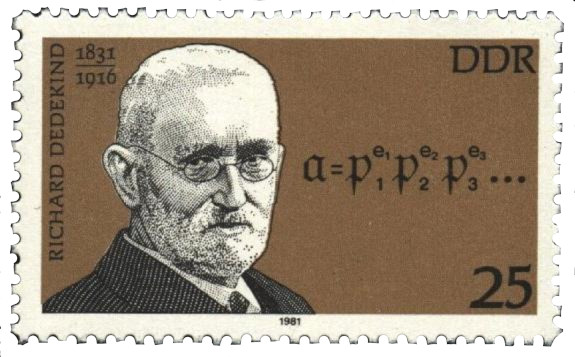
\includegraphics[width=7cm]{pic/Dedekind_stamp.jpg}
  \end{center}

  \caption{Estampilla de la República Democrática Alemana dedicada a Dedekind}
\end{figure}

%%%%%%%%%%%%%%%%%%%%%%%%%%%%%%%%%%%%%%%%%%%%%%%%%%%%%%%%%%%%%%%%%%%%%%%%%%%%%%%%

\pdfbookmark{Clase 5 (24/08/20)}{clase-5}
\section{Operaciones con ideales}
\marginpar{\small Clase 5 \\ 24/08/20}


Sea $R$ un anillo conmutativo. Ya hemos hablado de ideales principales en
el primer capítulo. En general, el ideal generado por elementos
$\alpha_1,\ldots,\alpha_n \in R$ viene dado por
\[ (\alpha_1,\ldots,\alpha_n) =
   \{ c_1 \alpha_1 + \cdots + c_n \alpha_n \mid c_1,\ldots,c_n \in R \}. \]
Los ideales de esta forma se llaman \textbf{finitamente generados}.

\begin{definicion}
  Para los ideales $I, J \subseteq R$ podemos considerar las siguientes
  operaciones.

  \begin{itemize}
  \item La \textbf{suma}
    $$I + J = \{ \alpha + \beta \mid \alpha \in I, \, \beta \in J \}$$
    es el ideal generado por los elementos de $I$ y $J$; en otras palabras,
    el ideal más pequeño que contiene a $I$ e $J$.

    En términos de generadores,
    \[ (\alpha_1,\ldots,\alpha_m) + (\beta_1,\ldots,\beta_n) =
       (\alpha_1,\ldots,\alpha_m,\beta_1,\ldots,\beta_n). \]

  \item El \textbf{producto}
    \[ IJ = \Bigl\{ \sum_{1 \le i \le n} \alpha_i \beta_i \Bigm|
                    n \ge 0, \, \alpha_i \in I, \, \beta_i \in J  \Bigl\} \]
    es el ideal generado por los productos $\alpha\beta$, donde $\alpha \in I$, $\beta \in J$.
    En términos de generadores,
    \[ (\alpha_1,\ldots,\alpha_m) \cdot (\beta_1,\ldots,\beta_n) =
       (\alpha_i \beta_j)_{\substack{1 \le i \le m \\ 1 \le j \le n}}. \]

    Notamos que se cumple $IJ \subseteq I\cap J$.
  \end{itemize}
\end{definicion}

Es fácil verificar que $+$ y $\cdot$ son operaciones asociativas y conmutativas
sobre ideales. Tenemos
$$I + (0) = I, ~ I + R = R, ~ I \cdot (0) = (0), ~ I\cdot R = I.$$
Además, se cumple la distributividad
$$(I + J) H = IH + JH$$
---dejo al lector verificar la doble inclusión.

Ya que hemos definido productos, podemos definir las potencias de la manera
habitual:
\[ I^0 = R, \quad
I^1 = I, \quad
I^2 = I\cdot I, \quad
I^3 = I\cdot I\cdot I, \quad
\ldots \]
Estas nos dan una cadena descendiente
$$R \supseteq I \supseteq I^2 \supseteq I^3 \supseteq \cdots$$

\begin{comentario}
  Cuidado: los elementos de $I^n$ no son productos de $n$ elementos de $I$
  (y mucho menos potencias $\alpha^n$ para $\alpha \in I$), sino \emph{sumas}
  de productos
  $$\sum_{i_1,\ldots,i_n} \alpha_{i_1} \cdots \alpha_{i_n}.$$
  Por ejemplo, en el anillo de polinomios $\ZZ [x]$, consideremos el ideal
  $I = (p,x)$. Entonces $p^2 + x^2 \in I$, pero este elemento no es de la forma
  $fg$ con $f,g \in I$.
\end{comentario}

Notamos que si $J = IH$ para algún $H$, entonces se tiene $J \subseteq H$.
Además, para los ideales principales se cumple
$$\alpha \mid \beta \iff (\alpha) \supseteq (\beta).$$
Esto justifica de alguna manera la siguiente definición.

\begin{definicion}
  Se dice que $I$ divide a $J$ (notación $I \mid J$) si $J \subseteq I$.
\end{definicion}

Sin embargo, hay que tener cuidado: en general no es cierto que $J \subseteq I$
siempre implica que $J = IH$ para algún ideal $H$. Vamos a ver un ejemplo
particular un poco más adelante.

\begin{definicion}
  Se dice que dos ideales $I,J \subseteq R$ son \textbf{coprimos} si
  $I + J = R$.
\end{definicion}

\begin{comentario}
  La motivación detrás del término ``coprimo'' es la siguiente:
  en un dominio de ideales principales (!) se tiene
  \[ (\alpha) + (\beta) = (\alpha,\beta) = (\gamma), \quad
     \text{donde }\gamma = \gcd (\alpha,\beta). \]
  Entonces, $\gcd (\alpha,\beta) = 1$ implica que $(\alpha)+(\beta) = R$.
 
  En general (si $R$ no es un dominio de ideales principales), esto es
  falso. Por ejemplo, en el anillo de polinomios $k[x,y]$ se tiene $\gcd (x,y)
  = 1$: los polinomios $x$ e $y$ claramente no tienen divisor en común (excepto
  constantes $c\ne 0$). Por otra parte, $(x,y) \ne k [x,y]$; de hecho,
  $k [x,y]/(x,y) \cong k$.

  Otro ejemplo, más relacionado con lo que estamos estudiando: en el anillo
  $\ZZ [\sqrt{-5}]$ consideremos el ideal $(2, 1 + \sqrt{-5})$. Sus dos
  generadores $2$ y $1 + \sqrt{-5}$ son elementos irreducibles no asociados
  entre sí, y por ende no tienen divisor en común. Sin embargo, no es difícil
  verificar que el ideal en cuestión es propio (y de hecho no es principal).
\end{comentario}

Ahora bien, ¿para qué sirven los ideales y operaciones aritméticas con ellos?
En el capítulo anterior hemos usado en algunas ocasiones que en un dominio
de factorización única, si $\gcd (\alpha,\beta) = 1$
y $\alpha\beta = \gamma^n$, entonces $\alpha$ y $\beta$ (salvo un múltiplo
invertible) son $n$-ésimas potencias: $\alpha \sim \alpha'^n$ y
$\beta \sim \beta'^n$.

Si no hay factorización única, esta propiedad falla.

\begin{ejemplo}
  Ya hemos notado que en el anillo $\ZZ [\sqrt{-5}]$ se tiene
  $$(2 + 3\sqrt{-5})\,(2 - 3\sqrt{-5}) = 7^2,$$
  donde $2 \pm 3\sqrt{-5}$ no es un cuadrado. Para corregir este defecto,
  se puede pasar a los ideales. Pongamos
  \[ I = (2 + 3\sqrt{-5}), \quad J = (2 - 3\sqrt{-5}), \quad H = (7). \]
  Tenemos
  $$I + J = R, \quad I J = H^2.$$
  Ahora
  $$(I + H)^2 = I^2 + I H + H^2 = I\,(I + H + J) = I,$$
  usando que $I + J = R$. De manera simétrica, $(J + H)^2 = J$. Entonces, aunque
  los números $2 \pm 3\sqrt{-5}$ no son cuadrados, los ideales principales
  generados por ellos sí lo son:
  $$(7, 2 \pm 3\sqrt{-5})^2 = (2 \pm 3\sqrt{-5}).$$
  El único detalle es que el ideal $(7, 2 \pm 3\sqrt{-5})$ no es principal;
  de manera contraria, tendríamos $2 \pm 3\sqrt{-5} = \pm\alpha^2$ para algún
  $\alpha$, pero no es el caso.
\end{ejemplo}

El truco de arriba funciona en general.

\begin{proposicion}
  \label{prop:producto-de-ideales-coprimos}
  Sean $I, J$ dos ideales tales que $I + J = R$ e $I J = H^n$.
  Entonces, $(I + H)^n = I$.

  \begin{proof}
    Primero una observación: si $I + J = R$, entonces $I^m + J = R$ para todo
    $m$. En efecto,
    \[ R = (I + J)^m =
       I^m + \underbrace{I^{m-1} J + \cdots + I J^{m-1} + J^m}_{\subseteq J}
       \subseteq I^m + J. \]

    Ahora
    \begin{align*}
      (I + H)^n & = I^n + I^{n-1} H + \cdots + I H^{n-1} + H^n \\
                & = I^n + I^{n-1} H + \cdots + I H^{n-1} + I J \\
                & = I\,(I^{n-1} + I^{n-2} H + \cdots + H^{n-1} + J) \\
                & = I,
    \end{align*}
    usando que $I^{n-1} + J = R$.
    \end{proof}
\end{proposicion}

Para terminar con la aritmética básica de ideales, revisemos el teorema chino
del resto. En un dominio de ideales principales este nos dice que
si $\gcd (\alpha,\beta) = 1$, entonces
$$R/(\alpha\beta) \cong R/(\alpha) \times R/(\beta).$$
En un anillo general, hay que considerar ideales coprimos. Primero hagamos
una pequeña observación

\begin{lema}
  Si $I + J = R$, entonces $I \cap J = IJ$.

  \begin{proof}
    Tenemos $IJ \subseteq I\cap J$ en cualquier caso. Ahora si $I + J = R$,
    escribamos $1 = \alpha + \beta$ para $\alpha \in I$, $\beta \in J$.
    Para todo $\gamma \in I \cap J$ se tiene entonces
    $$\gamma = \gamma\,(\alpha + \beta) = \gamma \alpha + \gamma \beta \in IJ.$$
    Esto demuestra la otra inclusión.
  \end{proof}
\end{lema}

Ahora el teorema chino del resto para anillos conmutativos es el siguiente
resultado.

\begin{teorema}[chino del resto]
  Sean $I, J \subseteq R$ ideales tales que $I + J = R$. Luego, hay un
  isomorfismo natural
  \begin{align*}
    R/(IJ) & \xrightarrow{\cong} R/I \times R/J,\\
    \alpha + IJ & \mapsto (\alpha + I, \alpha + J).
  \end{align*}

  \begin{proof}
    Consideremos el homomorfismo
    \[ \phi\colon R \to R/I \times R/J, \quad
       x \mapsto (x+I,x+J). \]
    Vamos a ver que es sobreyectivo y su núcleo es igual a $IJ$.

    Para ver la sobreyectividad, necesitamos probar que para cualesquiera
    $\alpha,\beta\in R$ existe $x\in I$ tal que
    $$x \equiv \alpha \pmod{I}, \quad x \equiv \beta \pmod{J}.$$
    De nuevo, dado que $I + J = R$, escribamos $a + b = 1$ para $a \in I$, $b
    \in J$. Notamos que
    \[ a \equiv 0 \pmod{I}, \quad
       a \equiv 1 \pmod{J}, \quad
       b \equiv 1 \pmod{I}, \quad
       b \equiv 0 \pmod{J}. \]
    Se ve que funcionará el elemento
    $$x = b \alpha + a \beta.$$

    En fin, está claro que $\ker \phi = I \cap J$, y por el lema anterior
    $I \cap J = IJ$.
  \end{proof}
\end{teorema}

\begin{comentario}
  La condición $I + J = R$ es necesaria para la prueba. Por ejemplo, si
  $I = J = 2\ZZ$, entonces $\ZZ/4\ZZ \not\cong \ZZ/2\ZZ \times \ZZ/2\ZZ$.
\end{comentario}

De manera similar, se puede probar que para una familia de ideales
$I_1,\ldots,I_n$ tales que $I_i + I_j = R$ para $i\ne j$, se tiene un isomorfismo
natural
$$R/(I_1\cdots I_n) \cong R/I_1 \times \cdots \times R/I_n$$
(he tomado $n = 2$ en la prueba se arriba solo para simplificar la notación).

\begin{ejemplo}
  Para un primo racional $p \equiv 1 \pmod{4}$ se tiene
  $p = \pi\,\overline{\pi}$ en $\ZZ[i]$. Ya que se trata de un dominio
  de ideales principales, se tiene
  $$(\pi) + (\overline{\pi}) = (\gcd (\pi, \overline{\pi})) = \ZZ[i],$$
  así que por el teorema chino del resto
  \[ \ZZ[i]/(p) \cong \ZZ[i]/(\pi) \times \ZZ[i]/(\overline{\pi})
                \cong \FF_p\times \FF_p. \]
  Otro modo de ver qué está pasando: tenemos
  $$\ZZ[i] \cong \ZZ[x]/(x^2+1), \quad \ZZ[i]/(p) \cong \FF_p [x]/(x^2+1).$$
  Ahora $x^2 + 1$ es irreducible o reducible en $\FF_p [x]$ dependiendo del
  símbolo de Legendre $\legendre{-1}{p} = \pm 1$. Cuando es reducible módulo $p$
  impar, salen dos diferentes factores lineales $x \pm a$, donde $a^2 \equiv -1
  \pmod{p}$.
\end{ejemplo}

%%%%%%%%%%%%%%%%%%%%%%%%%%%%%%%%%%%%%%%%%%%%%%%%%%%%%%%%%%%%%%%%%%%%%%%%%%%%%%%%

\section{Ideales primos y maximales}

El concepto que remplaza la noción de elemento primo es el de \emph{ideal} primo.

\begin{definicion}
  Se dice que un ideal $\mathfrak{p} \subset R$ es \textbf{primo} si este cumple
  una de las siguientes propiedades equivalentes:\footnote{Ejercicio:
    a)$\iff$a${}'$)$\iff$b).}
  \begin{enumerate}
  \item[a)] $\mathfrak{p} \ne R$ y si $\alpha\beta \in \mathfrak{p}$, entonces
    $\alpha \in \mathfrak{p}$ o $\beta \in \mathfrak{p}$;

  \item[a${}'$)] $\mathfrak{p} \ne R$ y si $IJ \subseteq \mathfrak{p}$, entonces
    $I \subseteq \mathfrak{p}$ o $J \subseteq \mathfrak{p}$;
  
  \item[b)] el anillo cociente $R/\mathfrak{p}$ es un dominio.
  \end{enumerate}

  El conjunto de los ideales primos en $R$ se llama el \textbf{espectro}
  de $R$ y se denota por
  $$\Spec R = \{ \mathfrak{p} \subset R \mid \text{ ideal primo} \}.$$

  Se dice que un ideal $\mathfrak{m} \subset R$ es \textbf{maximal} si este
  cumple una de las siguientes propiedades equivalentes:\footnote{Ejercicio:
    a)$\iff$b).}
  \begin{enumerate}
  \item[a)] $\mathfrak{m} \ne R$ y si $\mathfrak{m} \subseteq I \subseteq R$,
    entonces $I = \mathfrak{m}$ o $I = R$;

  \item[b)] el anillo cociente $R/\mathfrak{m}$ es un campo.
  \end{enumerate}
\end{definicion}
(Por la definición, el anillo nulo $R = 0$ no se considera como un dominio,
mucho menos como un campo.)

\begin{proposicion}
  Todo ideal maximal es primo.

  \begin{proof}
    Está claro de la caracterización b).
  \end{proof}
\end{proposicion}

\begin{ejemplo}
  Si $R$ es un dominio de ideales principales, entonces los ideales primos son
  $$\Spec R = \{ (0) \} \cup \{ (\pi) \mid \pi \in R \text{ es primo} \}.$$
  Los ideales de la forma $(\pi)$ son maximales, dado que $R/(\pi)$ es un campo.

  Para verlo, notamos que el ideal principal $(\pi) \subset R$ es primo si y
  solamente si $\pi \in R$ es un elemento primo en el sentido del capítulo
  anterior. En particular,
  \[ \Spec \ZZ = \{ (0) \} \cup \{ (2), (3), (5), (7), (11), \ldots \}. \qedhere \]
\end{ejemplo}

\begin{ejemplo}
  En el anillo $\ZZ [\sqrt{-5}]$ consideremos los ideales
  \[ \mathfrak{p} = (7, 3 + \sqrt{-5}), \quad
     \overline{\mathfrak{p}} = (7, 3 - \sqrt{-5}). \]

  Los ideales en cuestión no son principales: primero, analizando las normas se
  ve que $7$ y $3 \pm \sqrt{-5}$ son elementos irreducibles no asociados
  (las unidades son $\pm 1$). Luego, si $\mathfrak{p} = (\gamma)$, podemos
  considerar las expresiones
  $$7 = \alpha\gamma, \quad 3 + \sqrt{-5} = \beta\gamma$$
  para llegar a una contradicción. Dejo al lector los detalles.

  Estos ideales son coprimos:
  \[ 1 = 7 - (3 + \sqrt{-5}) - (3 - \sqrt{-5})
     \in \mathfrak{p} + \overline{\mathfrak{p}}. \]
  Su producto viene dado por
  \begin{align*}
    \mathfrak{p}\overline{\mathfrak{p}} & = (7, 3+\sqrt{-5})\,(7, 3-\sqrt{-5}) \\
    & = \Bigl(7^2, 7\,(3 + \sqrt{-5}), 7\,(3 - \sqrt{-5}), 14\Bigr) \\
    & = (7)\,(\underbrace{7, 3 + \sqrt{-5}, 3 - \sqrt{-5}, 2}_{= R}) = (7).
  \end{align*}

  Los ideales $\mathfrak{p}$ y $\overline{\mathfrak{p}}$ son propios.
  Por ejemplo, si $\mathfrak{p} = \ZZ [\sqrt{-5}]$, entonces
  para algunos $a,b,c,d \in \ZZ$ se tiene
  \[ 1 = (a + b\sqrt{-5})\cdot 7 + (c + d\sqrt{-5})\cdot (3 + \sqrt{-5})
       = (7a + 3c + 3d) + (7b + c + d)\sqrt{-5}. \]
  De la ecuación $7b + c + d = 0$ podemos expresar $d = -7b-c$,
  y luego al sustituirlo en $1 = 7a + 3c + 3d$ nos queda
  $1 = 7a - 21b$, pero el número a la derecha es par.

  Otra manera más lista es notar que el grupo
  $$\Gal (\QQ (\sqrt{-5})/\QQ) = \{ 1, \sigma \},$$
  donde $\sigma\colon \sqrt{-5} \mapsto -\sqrt{-5}$, actúa sobre
  $\ZZ [\sqrt{-5}]$. Para un ideal $I \subset \ZZ [\sqrt{-5}]$
  el conjunto $\sigma (I)$ es también un ideal, y además, en términos
  de generadores,
  \[ \sigma (\alpha_1,\ldots,\alpha_n) =
     (\sigma (\alpha_1), \ldots, \sigma (\alpha_n)). \]

  En nuestro caso particular se tiene
  $\overline{\mathfrak{p}} = \sigma (\mathfrak{p})$. Ahora si
  $\mathfrak{p} = \ZZ [\sqrt{-5}]$, entonces también
  $\overline{\mathfrak{p}} = \ZZ [\sqrt{-5}]$, pero en este caso
  $\mathfrak{p}\,\overline{\mathfrak{p}} = \ZZ [\sqrt{-5}]$, lo que
  contradice nuestro cálculo de arriba.

  Los ideales $\mathfrak{p}$ y $\overline{\mathfrak{p}}$ son maximales.
  Para verlo, podemos considerar el homomorfismo sobreyectivo
  \[ \phi\colon \ZZ[\sqrt{-5}] \to \FF_7 [x]/(3 + x), \quad
     a + b\sqrt{-5} \mapsto a + b\overline{x}. \]
  (Note que $3^2 \equiv -5 \pmod{7}$.)
  Tenemos $\ker\phi = \mathfrak{p}$, y este ideal es maximal.
  De manera similar se define un homomorfismo sobreyectivo
  $$\overline{\phi}\colon \ZZ[\sqrt{-5}] \to \FF_7 [x]/(3 - x),$$
  donde $\ker\overline{\phi} = \overline{\mathfrak{p}}$.

  Notamos que en general, un homomorfismo $\phi\colon \ZZ [\sqrt{-5}] \to \FF_7$
  está definido por la imagen de $\sqrt{-5}$ que debe cumplir
  $\phi (\sqrt{-5})^2 = -5$ en $\FF_p$. Las únicas posibilidades son
  $\phi (\sqrt{-5}) = \pm 3$, así que hemos encontrado los únicos dos ideales
  maximales que cumplen $\ZZ [\sqrt{-5}]/\mathfrak{p} \cong \FF_7$.

  El teorema chino del resto nos da en este caso
  \[ \begin{tikzcd}
    \ZZ [\sqrt{-5}]/(7) \ar{d}{\cong} &[-3em] \cong &[-3em] \ZZ[\sqrt{-5}]/\mathfrak{p} \ar{d}{\cong} &[-3em] \times &[-3em] \ZZ[\sqrt{-5}]/\overline{\mathfrak{p}} \ar{d}{\cong} \\
    \FF_7 [x]/(x^2 + 5) & \cong & \FF_7 [x]/(3 + x) \ar{d}{\cong} & \times & \FF_7 [x] / (3 - x) \ar{d}{\cong} \\
     && \FF_7 & \times & \FF_7
  \end{tikzcd} \]
\end{ejemplo}

\begin{proposicion}
  Un homomorfismo de anillos $\phi\colon S\to R$ induce una aplicación natural
  entre los espectros
  $$\phi^{-1}\colon \Spec R\to \Spec S, \quad
    \mathfrak{p} \mapsto \phi^{-1} (\mathfrak{p}).$$

  \begin{proof}
    Verifique si $\mathfrak{p} \subset R$ es un ideal primo, entonces
    $\phi^{-1} (\mathfrak{p})$ es un ideal primo en $S$.
  \end{proof}
\end{proposicion}

\begin{ejemplo}
  La inclusión natural $\ZZ \hookrightarrow \ZZ [\sqrt{-5}]$ induce
  una aplicación $\Spec \ZZ [\sqrt{-5}] \to \Spec \ZZ$ dada por
  $\mathfrak{p} \mapsto \mathfrak{p} \cap \ZZ$. En el ejemplo de arriba,
  \[ (7, 3 \pm \sqrt{-5}) \cap \ZZ = 7\ZZ. \qedhere \]
\end{ejemplo}

También nos servirá la siguiente propiedad.

\begin{proposicion}
  Dado un ideal propio $I \subsetneq R$, existe un ideal maximal
  $\mathfrak{m} \subset R$ tal que $I \subseteq \mathfrak{m}$.

  \begin{proof}
    Esta es una aplicación típica del lema de Zorn.

    Sea $\mathcal{P}$ el conjunto de los ideales propios
    $I \subseteq J_\alpha \subsetneq R$ parcialmente ordenado respecto a la
    inclusión $J_\alpha \subseteq J_\beta$. Un elemento maximal en $\mathcal{P}$
    sería precisamente un ideal maximal en $R$ que contiene a $I$. Para deducir
    la existencia de un elemento maximal, tenemos que probar que toda cadena en
    $\mathcal{P}$ es acotada.

    Una cadena en $\mathcal{P}$ es una colección de ideales propios
    $\mathcal{S} = \{ J_\alpha \mid I \subseteq J_\alpha \}$ donde
    $J_\alpha \subseteq J_\beta$ o $J_\beta \subseteq J_\alpha$ para
    cualesquiera $\alpha$ y $\beta$. La unión $J = \bigcup_\alpha J_\alpha$ es
    también un ideal propio en $R$. Este ideal $J$ nos da una cota superior para
    $\mathcal{S}$.
  \end{proof}
\end{proposicion}

Unos de los anillos más fáciles de manejar son anillos locales; más adelante
hablaremos de la localización, pero aquí está la definición de anillos locales.

\begin{definicion}
  Se dice que $R$ es un anillo \textbf{local} si $R$ tiene un único ideal
  maximal $\mathfrak{m}$. En este caso muy a menudo también se escribe
  ``$(R,\mathfrak{m})$ es local''.
\end{definicion}

\begin{ejemplo}
  El anillo
  $\ZZ_{(p)} = \Bigl\{ \frac{a}{b} \in \QQ \Bigm| p\nmid b \Bigr\}$
  es local: su único ideal maximal viene dado por $p\ZZ_{(p)}$.
  De una vez notamos que las unidades son
  $\ZZ_{(p)}^\times = \ZZ_{(p)}\setminus\mathfrak{m} = \Bigl\{ \frac{a}{b} \in \QQ \Bigm| p\nmid ab \Bigr\}$.
\end{ejemplo}

\begin{proposicion}
  Si $(R, \mathfrak{m})$ es un anillo local, entonces
  $R^\times = R\setminus \mathfrak{m}$.

  \begin{proof}
    Si $\alpha \notin R^\times$, entonces el ideal $(\alpha)$ es propio
    y está contenido en $\mathfrak{m}$ que es el único ideal maximal en este
    caso. Viceversa, un elemento $\alpha \in \mathfrak{m}$ no puede ser
    invertible, dado que $\mathfrak{m} \ne R$.
  \end{proof}
\end{proposicion}

Notamos que viceversa, si todos los elementos no-invertibles de $R$ forman un
ideal, entonces este es maximal y $R$ es un anillo local.

%%%%%%%%%%%%%%%%%%%%%%%%%%%%%%%%%%%%%%%%%%%%%%%%%%%%%%%%%%%%%%%%%%%%%%%%%%%%%%%%

\section{Ideales en anillos de números}

Sea $R$ un anillo de números.

\begin{lema}
  Para todo ideal no nulo $I \subseteq R$ se tiene $I \cap \ZZ \ne (0)$.

  \begin{proof}
    Si $\alpha \in I$ es un elemento no nulo, entonces $\alpha$, siendo un
    número algebraico (!), satisface una relación algebraica no trivial
    $$a_n \alpha^n + \cdots + a_1 \alpha + a_0 = 0,$$
    donde $a_i \in \ZZ$, y sin pérdida de generalidad, $a_0 \ne 0$. Entonces,
    $a_0 \in I$.
  \end{proof}
\end{lema}

\begin{corolario}
  Para todo ideal primo no nulo $\mathfrak{p} \subset R$ se tiene
  $\mathfrak{p} \cap \ZZ = p\ZZ$ para algún primo racional $p$.

  \begin{proof}
    La intersección $\mathfrak{p} \cap \ZZ$ debe ser un ideal primo no nulo en
    $\ZZ$.
  \end{proof}
\end{corolario}

\begin{teorema}
  \label{thm:R/I-finito}
  Para todo ideal no nulo $I \subset R$ el cociente $R/I$ es finito.

  \begin{proof}
    Consideremos $R/I$ como un grupo abeliano ($\ZZ$-módulo). Un subgrupo
    finitamente generado de $R/I$ corresponde a un subgrupo finitamente generado
    $M \subseteq R$ tal que $I \subseteq M$.

    Dado que $M \subset K$, donde $K/\QQ$ es un campo de números, $M$ no tiene
    torsión y por ende es un $\ZZ$-módulo libre de rango $r$:
    $$M \cong \underbrace{\ZZ\oplus\cdots\oplus\ZZ}_r.$$
    Notamos que más de $[K : \QQ]$ elementos de $M$ tendrían una dependencia
    $\QQ$-lineal (¡y luego $\ZZ$-lineal!) no trivial.  Esto implica que
    $r \le [K : \QQ]$.

    Denotemos por $M/I$ la imagen de $M$ en el cociente $R/I$.
    Como vimos arriba, $n \in I$ para algún entero $n > 0$, y luego
    $$\# (M/I) \le \# (M/(n)) \le n^{[K : \QQ]}.$$

    Entonces, acabamos de probar que todo subgrupo finitamente generado
    $M/I \subset R/I$ es finito, y además $\# (M/I) \le C$ para cierta constante
    $C$ que no depende de $M$. Esto significa qe $R/I$ es finito.
  \end{proof}
\end{teorema}

\begin{comentario}
  Los argumentos de arriba usan que $R$ es un anillo de números. Sino, podemos
  tomar por ejemplo $R = \ZZ[x]$ y el ideal $\mathfrak{p} = (x)$. Se tiene
  entonces $R/\mathfrak{p} \cong \ZZ$ y $\mathfrak{p} \cap \ZZ = (0)$.

  En este caso $R \subset K$, donde $K = \QQ (x)$, pero la extensión $K/\QQ$
  es infinita de grado de trascendencia $1$.
\end{comentario}

\pdfbookmark{Clase 6 (26/08/20)}{clase-6}
\marginpar{\small Clase 6 \\ 26/08/20}

Después de definir el anillo de enteros $\O_K$, vamos a establecer algunas
de sus propiedades básicas.

\begin{corolario}
  Todo anillo de números $R$ es noetheriano.

  \begin{proof}
    Para dos ideales no nulos $I\subsetneq J\subseteq R$ tenemos un homomorfismo
    sobreyectivo natural ${R/I\twoheadrightarrow R/J}$,
    y luego $\# (R/J) < \# (R/I) < \infty$.  Esto implica que no puede existir
    una cadena infinita ascendente
    \[ I_0 \subsetneq I_1 \subsetneq I_2 \subsetneq \cdots \qedhere \]
  \end{proof}
\end{corolario}

\begin{corolario}
  Todo ideal primo no nulo $\mathfrak{p} \subset R$ es maximal.

  \begin{proof}
    El anillo cociente $R/\mathfrak{p}$ es un dominio finito, pero recordemos
    que todo dominio finito es un campo.\footnote{Si $D$ es un dominio finito,
      entonces para todo elemento no nulo $a \in D$ la multiplicación por $a$
    $$\mu_a\colon D \to D, \quad x \mapsto ax$$ es una aplicación
    inyectiva. Dado que $D$ es finito, $\mu_a$ es también sobreyectiva y existe
    $a^{-1} \in D$ tal que $\mu_a (a^{-1}) = a a^{-1} = 1$.}
  \end{proof}
\end{corolario}

\begin{corolario}
  Si para dos ideales primos no nulos $\mathfrak{p}, \mathfrak{q} \subset R$ se
  tiene $\mathfrak{p} \subseteq \mathfrak{q}$, entonces $\mathfrak{p} =
  \mathfrak{q}$.
\end{corolario}

\begin{definicion}
  Para un anillo conmutativo $R$ la \textbf{dimensión de Krull} viene dada por
  \[ \dim R =
     \sup \{ n \mid \text{existe una cadena de ideales primos }
             \mathfrak{p}_0 \subsetneq \mathfrak{p}_1 \subsetneq \cdots
             \subsetneq{p}_n \subset R \}. \]
\end{definicion}

Por ejemplo, todo campo $k$ tiene el único ideal $(0)$, así que $\dim k = 0$.

Si $R$ es un anillo de números que no es un campo, entonces $\dim R = 1$ por lo
que acabamos de probar: la cadena más larga de ideales primos tiene forma
$(0) \subsetneq \mathfrak{p} \subset R$. Esto significa que $R$ es un objeto
unidimensional, y esto explica muchas buenas propiedades.

\begin{ejemplo}
  En general, se puede probar que para los anillos de polinomios
  $$\dim R [x_1,\ldots,x_n] = \dim R + n.$$
  En particular, si $k$ es un campo, $\dim k [x_1,\ldots,x_n] = n$.
  Esto corresponde al hecho geométrico de que el espacio afín
  $\AA^n (k)$ tiene dimensión $n$.

  De la misma manera, $\dim \ZZ[x] = 2$, dado que $\dim \ZZ = 1$.

  Para más información sobre la dimensión de Krull, véanse los libros de texto
  de álgebra conmutativa.
\end{ejemplo}

Ahora bien, dado un anillo de números $R \subset K$ y un ideal primo no nulo
(= maximal) $\mathfrak{p} \subset R$, tenemos $\ZZ \cap \mathfrak{p} = p\ZZ$ para
algún primo racional $p$, y el \textbf{campo residual} $R/\mathfrak{p}$ es una
extensión de $\FF_p$ de grado finito $f_\mathfrak{p} \le [K : \QQ]$.

\[ \begin{tikzcd}
&[-3em] &[-3em] \mathfrak{p} &[-3em] \subset &[-3em] R \ar[->>]{r}\ar[-]{d} & R/\mathfrak{p} \ar[-]{d}{f_\mathfrak{p}} \\
\mathfrak{p} \cap \ZZ & = & (p) & \subset & \ZZ \ar[->>]{r} & \FF_p
\end{tikzcd} \]

\begin{ejemplo}
  El siguiente dibujo representa los ideales primos en el anillo $R = \ZZ [i]$ a
  través de la aplicación $\Spec \ZZ [i] \to \Spec \ZZ$. Aquí todo primo no nulo
  $\mathfrak{p} \subset R$ está sobre algún primo racional $p \in \ZZ$.  Los
  ``puntos gruesos'' en el dibujo representan los ideales primos nulos $(0)$.

  \begin{center}
    \includegraphics{pic/SpecZi.pdf}
  \end{center}

  Lo que vimos en el capitulo anterior puede ser resumido de la siguiente
  manera.
  \begin{enumerate}
  \item[1)] Se tiene $2\ZZ [i] = \mathfrak{p}^2$, donde $\mathfrak{p} = (1+i)$.
    En este caso $f = 1$.

  \item[2)] Si $p \equiv 1 \pmod{4}$, entonces
    $p\ZZ [i] = \mathfrak{p} \,\overline{\mathfrak{p}}$
    para dos diferentes primos $\mathfrak{p},\overline{\mathfrak{p}}$.
    Aquí $f_\mathfrak{p} = f_{\overline{\mathfrak{p}}} = 1$.

  \item[3)] Si $p \equiv 3 \pmod{4}$, entonces $p\ZZ [i]$ es primo, y en este
    caso $f = 2$. \qedhere
  \end{enumerate}
\end{ejemplo}

%%%%%%%%%%%%%%%%%%%%%%%%%%%%%%%%%%%%%%%%%%%%%%%%%%%%%%%%%%%%%%%%%%%%%%%%%%%%%%%%

\section{Ideales fraccionarios}

Hemos visto cómo sumar y multiplicar los ideales. Estas operaciones cumplen
varias propiedades parecidas a los axiomas de anillo conmutativo, pero para un
ideal $I$ no existe el ideal ``$-I$'' que cumpliría $I + (-I) = (0)$. De hecho,
no hay manera razonable de añadirlo: en ese caso la identidad $I + I = I$
implicaría que $R = (0)$. Pero lo que sí se puede tratar de hacer es añadir los
ideales inversos $I^{-1}$ que cumplen $I I^{-1} = R$.

Por ejemplo, el ideal inverso a $2\ZZ \subset \ZZ$ debería de ser algo como
$\frac{1}{2}\ZZ$, pero $\frac{1}{2}$ no vive en $\ZZ$, sino en su
campo de fracciones $\QQ$. Esto nos lleva a la noción de ideales fraccionarios.

Aunque el material de la sección anterior es válido para cualquier anillo
conmutativo, pero a partir de ahora tendremos que suponer que $R$ es
un dominio. Denotemos por $K$ el campo de fracciones de $R$.

\begin{definicion}
  Un $R$-\textbf{ideal fraccionario} es un $R$-submódulo $I \subseteq K$
  que cumple la siguiente propiedad: existe $\alpha \in K^\times$ tal que
  $\alpha I \subseteq R$.

  Se dice que $I$ es \textbf{principal} si $I = \alpha R$ para algún
  $\alpha \in K^\times$.

  Si $I \subseteq R$, entonces $I$ es un ideal en el sentido normal, y para
  subrayar este hecho se dice que $I$ es un ideal \textbf{entero}.
\end{definicion}

La condición $\alpha I \subseteq R$ significa lo siguiente: aunque en $I$ pueden
estar fracciones, sus denominadores deben ser controlables y cancelarse
al multiplicar $I$ por un solo elemento.

\begin{ejemplo}
  Consideremos $R = \ZZ$. En este caso $K = \QQ$. Si $\alpha I$ es un subgrupo
  de $\ZZ$, entonces $\alpha I = n\ZZ$ para algún número natural $n$. Luego,
  $I = \alpha^{-1} n \ZZ$, donde $\alpha^{-1} n \in \QQ$. Entonces, los ideales
  fraccionarios de $\ZZ$ son de la forma $\frac{a}{b} \ZZ$, donde
  $\frac{a}{b} \in \QQ$. Todos son principales.

  Hay muchos más $\ZZ$-submódulos $I \subseteq \QQ$, como por ejemplo
  $\ZZ \Bigl[\frac{1}{2}\Bigr]$, pero estos no cumplen la condición
  $\alpha I \subseteq \ZZ$.
\end{ejemplo}

El ejemplo de arriba funciona de manera similar en cualquier dominio de ideales
principales.

Las operaciones $I + J$, $I \cap J$, $IJ$ definidas para los ideales enteros
en la sección anterior se definen de la misma manera para los ideales
fraccionarios (se deja como un ejercicio verificar que el resultado es también
un ideal fraccionario).

\begin{definicion}
  Se dice que un $R$-ideal fraccionario $I$ es \textbf{invertible} si existe
  otro ideal fraccionario $J$ tal que $IJ = R$.
\end{definicion}

\begin{proposicion}
    Si $I$ es invertible, entonces su inverso es igual a
    $$I^{-1} = \{ \alpha \in K \mid \alpha I \subseteq R \}.$$
    Entonces, $I$ es invertible si y solamente si $I I^{-1} = R$.

    \begin{proof}
      Notamos que $II^{-1} \subseteq R$. Ahora si $IJ = R$, entonces se ve que
      $J \subseteq I^{-1}$. Por otra parte,
      $I^{-1} = I^{-1}\cdot IJ = (I^{-1} I)\cdot J \subseteq RJ = J$.
    \end{proof}
\end{proposicion}

\begin{ejemplo}
  Todo ideal fraccionario principal es invertible: para $\alpha \in K^\times$ se
  tiene $(\alpha R)^{-1} = \alpha^{-1} R$.
\end{ejemplo}

No todos los ideales en un anillo de números es invertible. He aquí un ejemplo
particular.

\begin{ejemplo}
  \label{ejemplo:Z-sqrt-m3-ideal-no-invertible}
  Consideremos el ideal $\mathfrak{p} = (2, 1+\sqrt{-3})$ en el anillo
  $R = \ZZ [\sqrt{-3}]$. Se tiene $R/\mathfrak{p} \cong \FF_2$, así que
  se trata de un ideal maximal. Su inverso tendría que ser
  \[ \mathfrak{p}^{-1} = \{ \alpha \in \QQ (\sqrt{-3}) \mid
                           2 \alpha \in \ZZ [\sqrt{-3}],
                           (1+\sqrt{-3})\,\alpha \in \ZZ [\sqrt{-3}] \}. \]

  Escribiendo $\alpha = a+b\sqrt{-3}$, notamos que la primera condición
  significa que $a = a'/2$, $b = b'/2$ para $a', b' \in \ZZ$.
  Para la segunda condición, calculamos que
  \[ (1 + \sqrt{-3}) \, \Bigl(\frac{a'}{2} + \frac{b'}{2}\sqrt{-3}\Bigr) =
     \frac{a' - 3b'}{2} + \frac{a' + b'}{2}\,\sqrt{-3}. \]
  Este elemento está en $\ZZ [\sqrt{-3}]$ si y solamente si
  $a' \equiv b' \pmod{2}$. Podemos concluir que
  \[ \mathfrak{p}^{-1} =
     \Bigl\{ \frac{a'}{2} + \frac{b'}{2}\sqrt{-3} \Bigm|
             a',b' \in \ZZ, a' \equiv b' (2) \Bigr\}
     \stackrel{\text{Ejercicio}}{=} \ZZ \Bigl[\frac{1+\sqrt{-3}}{2}\Bigr]. \]

  Ahora, usando $\frac{(1 + \sqrt{-3})^2}{2} = -1 + \sqrt{-3}$, tenemos
  $$\mathfrak{p} \mathfrak{p}^{-1} =
    (2, 1 + \sqrt{-3}) \, \Bigl(1, \frac{1 + \sqrt{-3}}{2}\Bigr) =
    (2, 1 + \sqrt{-3}, -1 + \sqrt{-3}) = \mathfrak{p} \ne R.$$

  Por otra parte, en el anillo más grande
  $\ZZ \Bigl[\frac{1+\sqrt{-3}}{2}\Bigr] = \ZZ [\zeta_3]$
  (que es un dominio de ideales principales, como ya sabemos) tenemos
  $\mathfrak{p} = (2)$.
\end{ejemplo}

\iffalse
\begin{ejemplo}
  \label{ejemplo:primo-no-invertible-Z-sqrt-8}
  Consideremos el anillo
  \[ \begin{tikzcd}[row sep=1em]
    R &[-3em] = &[-3em] \ZZ [\sqrt{8}]\ar[equals]{d} &[-3em] \subsetneq &[-3em] \ZZ [\sqrt{2}]\ar[equals]{d} \\
    & & \ZZ \oplus 2\sqrt{2}\ZZ & \subsetneq & \ZZ \oplus \sqrt{2}\ZZ
  \end{tikzcd} \]

  Tomemos la cadena de ideales
  \[ \begin{tikzcd}[row sep=0.5em]
    \mathfrak{p}^2\ar[equals]{d} &[-2em] \subsetneq &[-2em] I\ar[equals]{d} &[-2em] \subsetneq &[-2em] \mathfrak{p}\ar[equals]{d} &[-2em] \subsetneq &[-2em] R\ar[equals]{d} \\
    4\ZZ \oplus 4\sqrt{2}\ZZ &  \stackrel{2}{\subsetneq} & 2\ZZ \oplus 4\sqrt{2}\ZZ & \stackrel{2}{\subsetneq} & 2\ZZ \oplus \sqrt{2}\ZZ & \stackrel{2}{\subsetneq} & \ZZ \oplus 2\sqrt{2}\ZZ
  \end{tikzcd} \]

  Aquí $I \subseteq \mathfrak{p}$, así que por nuestra definición $\mathfrak{p}
  \mid I$. ¿Será cierto que $I = \mathfrak{p} J$ para algún ideal
  $J \subseteq R$?

  En este caso dado que $I \subsetneq \mathfrak{p}$, tenemos
  $J \subsetneq R$. Sea $\mathfrak{q}$ un ideal maximal tal que
  $J \subseteq \mathfrak{q}$. Se tiene
  $$\mathfrak{p}^2 \subset I = \mathfrak{p} J \subseteq J \subseteq \mathfrak{q},$$
  y luego $\mathfrak{p} \subseteq \mathfrak{q}$. Pero esto
  implica que $\mathfrak{p} = \mathfrak{q}$. Ahora
  $I = \mathfrak{p} J \subseteq \mathfrak{p}^2$, lo que nos da una
  contradicción.

  Entonces, aunque $I \subset \mathfrak{p}$, no existe ningún ideal $J$ tal que
  $I = \mathfrak{p} J$. Si $\mathfrak{p}$ fuera invertible, bastaría tomar
  $J = \mathfrak{p}^{-1} I$, pero lo que acabamos de ver demuestra que
  $\mathfrak{p}$ no es invertible.
\end{ejemplo}
\fi

\begin{definicion}
  Denotemos por $\mathcal{I} (R)$ el grupo de $R$-ideales fraccionarios
  invertibles y por $\mathcal{P} (R)$ el subgrupo de $R$-ideales fraccionarios
  principales. Luego, el \textbf{grupo de Picard} de $R$ es el cociente
  $$\Pic (R) = \mathcal{I} (R) / \mathcal{P} (R).$$
\end{definicion}

Aunque los ideales invertibles forman un grupo abeliano respecto
a \emph{multiplicación}, muy a menudo $\Pic (R)$ se escribe en la notación
aditiva. La definición puede ser resumida en la \textbf{sucesión exacta}
de grupos abeluanos.
\[ 1 \to R^\times \to K^\times \xrightarrow{\alpha \mapsto \alpha R}
       \mathcal{I} (R) \to \Pic (R) \to 0 \]

\begin{ejemplo}
  Para todo dominio de ideales principales se tiene $\Pic (R) = 0$.
\end{ejemplo}

\begin{ejemplo}
  Para todo anillo local $(R,\mathfrak{m})$ se tiene $\Pic (R) = 0$.

  \begin{proof}
    Sea $I$ un $R$-ideal fraccionario invertible. En este caso la ecuación
    $I I^{-1} = R$ significa que se puede escribir
    $$\sum_i \alpha_i \beta_i = 1,$$
    donde $\alpha_i \in I$ y $\beta_i \in I^{-1}$. Tenemos necesariamente
    $\alpha_i \beta_i \in R^\times$ para algún $i$; en el caso contrario
    $\sum_i \alpha_i \beta_i$ está en el ideal maximal
    $\mathfrak{m} = R\setminus R^\times$ (es aquí donde estamos usando que $R$
    es local). Ahora $\beta_i I = R$, así que $I = (\beta_i^{-1})$ es principal.
  \end{proof}
\end{ejemplo}

Uno de los resultados principales del curso establece la finitud de $\Pic (R)$
para todo orden $R \subset K$. También veremos cómo hacer cálculos particulares.

\begin{ejemplo}
  Consideremos el anillo $R = \ZZ [\sqrt{-5}]$. El ideal
  $$\mathfrak{p} = (2, 1 + \sqrt{-5})$$
  no es principal. Por ejemplo, podemos calcular que
  \[ \mathfrak{p}^2 = (2^2, 2\,(1 + \sqrt{-5}), (1 + \sqrt{-5})^2)
     = (2) \, (\underbrace{2, 1 + \sqrt{-5}, -2 + \sqrt{-5}}_{= R}) = 2R.\]
  Ahora si $\mathfrak{p}$ fuera principal, esto nos daría $2 \sim \alpha^2$
  para algún $\alpha$, pero $2$ es irreducible en el anillo $\ZZ [\sqrt{-5}]$.

  El ideal es maximal: tenemos $R/\mathfrak{p} \cong \FF_2$.
  De una vez hemos calculado que $\mathfrak{p}$ es invertible: su inverso es
  \[ \mathfrak{p}^{-1} = \frac{1}{2}\mathfrak{p}
     = \Bigl(1, \frac{1 + \sqrt{-5}}{2}\Bigr). \]

  Dado que $\mathfrak{p}^2 = 2R$ es principal, $[\mathfrak{p}]$ es un elemento
  de orden $2$ en el grupo de Picard. De hecho,
  $\Pic (\ZZ [\sqrt{-5}]) \cong \ZZ/2\ZZ$, donde $\mathfrak{p}$ representa el
  generador. Para justificar este calculo necesitamos varias herramientas que
  veremos más adelante en el curso.

  Solo para dar un ejemplo de cómo se comportan los ideales en este caso,
  $\mathfrak{q} = (3, 1 + \sqrt{-5})$ es también un ideal que no es principal.
  El lector puede verificar que
  \[ \mathfrak{q}\,\overline{\mathfrak{q}} = 3R, \quad
     \ZZ [\sqrt{-5}]/\mathfrak{q} \cong \FF_3. \]

  Para $\alpha = \frac{1-\sqrt{-5}}{3}$ tenemos
  \[ (\alpha)\,\mathfrak{q} =
     \left(\frac{1-\sqrt{-5}}{3}\right) \, (3, 1 + \sqrt{-5}) =
     (2, 1-\sqrt{-5}) = (2, 1+\sqrt{-5}) = \mathfrak{p}. \]
  Entonces, $[\mathfrak{q}] = [\mathfrak{p}]$ en $\Pic (\ZZ [\sqrt{-5}])$.
\end{ejemplo}

El grupo de Picard puede ayudar a resolver ecuaciones diofánticas.

\begin{ejemplo}
  Continuando con el ejemplo anterior, consideremos la curva elíptica
  $$y^2 = x^3 - 5.$$
  Afirmamos que esta no tiene putos enteros.

  Primero, $y$ tiene que ser par. Por ejemplo, reduciendo la ecuación módulo
  $4$, notamos que $x^3 - 5 \not\equiv 1 \pmod{4}$. Además, $y \ne 0$.

  Como hacíamos antes, empezamos por escribir
  $$x^3 = (y - \sqrt{-5})\,(y + \sqrt{-5}).$$
  El anillo $\ZZ [\sqrt{-5}]$ no es un dominio de factorización única,
  pero vamos a trabajar con ideales en lugar de elementos.

  Afirmamos que para $y \ne 0$ par se tiene
  $$(y - \sqrt{-5}, y + \sqrt{-5}) = \ZZ [\sqrt{-5}].$$
  Primero calculamos que
  \[ \left(\frac{y}{2} - \sqrt{-5}\right) \cdot (y + \sqrt{-5})
       - \frac{y}{2}\cdot (y - \sqrt{-5}) = 5
     \in (y - \sqrt{-5}, y + \sqrt{-5}). \]
  Además, está claro que
  $$2y \in (y - \sqrt{-5}, y + \sqrt{-5}).$$

  Por otro lado, se ve que $5 \nmid y$: para esto considere la ecuación
  $y^2 = x^3 - 5$ y fíjese en la valuación $v_5 (\cdot)$. Tenemos entonces
  $\gcd (2y, 5) = 1$, así que
  $(y - \sqrt{-5}, y + \sqrt{-5}) = \ZZ [\sqrt{-5}]$.

  Ahora $(y + \sqrt{-5})$ e $(y - \sqrt{-5})$ son ideales coprimos y su producto
  es $(x)^3$, así que gracias a \ref{prop:producto-de-ideales-coprimos} debe
  existir un ideal $I \subset R$ tal que
  $$(y + \sqrt{-5}) = I^3$$
  Aquí el ideal a la izquierda es principal, así que $[I^3]$ es trivial en
  $\Pic (\ZZ [\sqrt{-5}])$. Pero sabiendo que el grupo de Picard tiene orden
  $2$, esto nos permite concluir que $[I]$ es trivial; es decir, un ideal
  principal. Escribiendo $I = (a + b\sqrt{-5})$, se obtiene
  $$y + \sqrt{-5} = (a + b\sqrt{-5})^3 = a\,(a^2 - 15\,b^2) + b\,(3a^2 - 5b^2).$$
  Pero la ecuación $b\,(3a^2 - 5b^2) = 1$ no tiene soluciones enteras, así que
  podemos concluir que $y^2 = x^3 + 5$ tampoco tiene soluciones enteras.
\end{ejemplo}

Cabe mencionar que en geometría algebraica también existe la noción del grupo de
Picard de una curva que se define de manera parecida como el cociente del grupo
de divisores por los divisores principales. Véase
\cite[Chapter II]{Silverman-GTM106} o \cite{Lorenzini-1996} para mayor
información.

%%%%%%%%%%%%%%%%%%%%%%%%%%%%%%%%%%%%%%%%%%%%%%%%%%%%%%%%%%%%%%%%%%%%%%%%%%%%%%%%

\section{Anillo de enteros $\O_K$}

Siguiendo con nuestro programa de llevar la aritmética de elementos
$\alpha \in R$ a la aritmética de ideales $I \subset R$, una propiedad que nos
gustaría tener es el teorema fundamental de la aritmética que para los ideales
quiere decir que todo ideal propio no nulo $I \subset R$ se descompone en
producto de ideales primos
$$I = \mathfrak{p}_1^{e_1}\cdots \mathfrak{p}_s^{e_s},$$
donde los elementos $e_i$ están definidos de modo único.
Desgraciadamente, esto no es siempre posible en un anillo de números.

\begin{ejemplo}
  Consideremos el anillo $R = \ZZ [\sqrt{-3}]$ y el ideal
  $\mathfrak{p} = (2, 1+\sqrt{-3})$.  Calculamos que
  \[ \mathfrak{p}^2 = (2^2, 2\,(1+\sqrt{-3}), (1 + \sqrt{-3})^2) =
     2R\cdot (2, 1+\sqrt{-3}, -1 + \sqrt{-3}) = 2R\cdot \mathfrak{p}. \]
  Si tuviéramos la factorización única, esto implicaría que $\mathfrak{p} = 2R$.
  Sin embargo,
  \[ \tag{*} R \supset \mathfrak{p} \supsetneq 2R \supsetneq \mathfrak{p}^2
     \supset \mathfrak{p}^3 \supset \mathfrak{p}^4 \supset \cdots \]
 
  Aún peor, el ideal $2R$ no puede ser escrito como un producto de ideales
  primos. Para verlo, supongamos que para algunos ideales primos $\mathfrak{p}_i$
  se cumple
  $$2R = \mathfrak{p}_1^{e_1} \cdots \mathfrak{p}_s^{e_s}.$$
  Luego, tenemos
  $$\mathfrak{p}^2 \subsetneq 2R \subseteq \mathfrak{p}_i.$$
  Esto implica que $\mathfrak{p} \subseteq \mathfrak{p}_i$ por la primalidad de
  $\mathfrak{p}_i$, pero luego $\mathfrak{p}_i = \mathfrak{p}$, dado que
  $\mathfrak{p}$ es un ideal maximal. Esto significa que $2R = \mathfrak{p}^n$
  para algún $n$, pero esto contradice (*). Entonces, ¡el ideal $2R$ no es un
  producto de ideales primos!
\end{ejemplo}

El ideal $\mathfrak{p}$ de arriba no es invertible, como ya vimos en
\ref{ejemplo:Z-sqrt-m3-ideal-no-invertible}. Resulta que si queremos
descomposiciones en productos de ideales primos, no pueden existir ideales no
invertibles.

\begin{proposicion}
  \label{prop:factorizacion-en-primos-invertibilidad}
  Sea $R$ un anillo de números donde todo ideal propio no nulo $I \subset R$
  puede ser escrito como producto de ideales primos
  $$I = \mathfrak{p}_1^{e_1}\cdots \mathfrak{p}_s^{e_s}.$$
  Entonces, todo $R$-ideal fraccionario es invertible.

  \begin{proof}
    Bajo la hipótesis, bastaría verificar que todo ideal primo no nulo
    $\mathfrak{p} \subset R$ es invertible. Consideremos un elemento no
    nulo $\alpha \in \mathfrak{p}$ y la descomposición
    $$\alpha R = \mathfrak{p}_1^{e_1}\cdots\mathfrak{p}_s^{e_s}.$$
    Los ideales $\mathfrak{p}_i$ son primos no nulos, y entonces maximales.
    Aquí todos los ideales $\mathfrak{p}_i$ son invertibles:
    \[ \mathfrak{p}_i^{-1} =
       \frac{1}{\alpha}R \mathfrak{p}_1^{e_1}\cdots
       \mathfrak{p}_i^{e_i - 1}\cdots\mathfrak{p}_s^{e_s}. \]
    Tenemos
    $$\mathfrak{p}_1^{e_1}\cdots\mathfrak{p}_s^{e_s} \subseteq \mathfrak{p},$$
    pero por la primalidad de $\mathfrak{p}$ y maximalidad de los
    $\mathfrak{p}_i$, tenemos $\mathfrak{p} = \mathfrak{p}_i$, así que es
    invertible.
  \end{proof}
\end{proposicion}

Ahora ¿qué defecto tiene el anillo $\ZZ [\sqrt{-3}]$ que nos da ideales no
invertibles? En $\QQ (\sqrt{-3}) = \Frac \ZZ [\sqrt{-3}]$ tenemos el entero
algebraico $\alpha = \frac{1+\sqrt{-3}}{2}$: este cumple la relación mónica
$$\alpha^2 - \alpha + 1 = 0.$$
Ahora consideremos el ideal fraccionario
$$I = (1, \alpha).$$
Calculamos que
$$I^2 = (1, \alpha, \alpha^2) = (1, \alpha) = I.$$
Si $I$ fuera invertible, multiplicando esta ecuación por $I^{-1}$ tendríamos
$I = R$, pero esto no es el caso. Este truco funciona en general. Será oportuno
dar una definición.

\begin{definicion}
  Sea $R$ un dominio. Se dice que $\alpha \in \Frac (R)$
  es \textbf{entero} sobre $R$ si existe una relación mónica
  $$\alpha^n + a_{n-1} \alpha^{n-1} + \cdots + a_1 \alpha + a_0 = 0,$$
  donde $a_i \in R$. Si todo elemento entero sobre $R$ está en $R$,
  entonces se dice que $R$ es \textbf{integralmente cerrado}.
\end{definicion}

Por ejemplo, el anillo $\ZZ [\sqrt{-3}]$ no es integralmente cerrado porque no
contiene el elemento $\frac{1+\sqrt{-3}}{2}$. Resulta que esta es la raíz de los
problemas.

\begin{proposicion}
  Sea $R$ un anillo de números donde todo $R$-ideal fraccionario es invertible.
  Entonces, $R$ es integralmente cerrado en $\Frac (R)$.

  \begin{proof}
    Sea $\alpha \in \Frac (R)$ un elemento no nulo que satisface una relación
    mónica
    $$\alpha^n + a_{n-1} \alpha^{n-1} + \cdots + a_1 \alpha + a_0 = 0,$$
    donde $a_i \in R$. Consideremos el ideal fraccionario
    $$I = (1,\alpha,\alpha^2,\ldots,\alpha^{n-1}).$$
    Gracias a la relación de arriba, toda potencia $\alpha^k$ para $k \ge n$
    se expresa como una combinación $\ZZ$-lineal de $1,\alpha,\ldots,\alpha^n$,
    y se ve que
    $$I^2 = I.$$
    Ahora si $I$ es invertible, entonces $I = R$, y en particular
    $\alpha \in R$.
  \end{proof}
\end{proposicion}

Ahora sabiendo la importancia de anillos integralmente cerrados, vamos
a investigar este concepto.

\begin{lema}[Caracterización de integralidad]
  \label{lema:caracterizacion-de-integralidad}
  Sea $K$ un campo y $R \subset K$ un subanillo.
  Para $\alpha \in K$ las siguientes condiciones son equivalentes.

  \begin{enumerate}
  \item[a)] $\alpha$ es entero sobre $R$.

  \item[b)] $R [\alpha] \subset K$ es un $R$-módulo finitamente generado.

  \item[c)] Existe un $R$-módulo finitamente generado no nulo
    $M \subseteq K$ tal que $\alpha M \subseteq M$.
  \end{enumerate}

  \begin{proof}
    \noindent a)$\Rightarrow$b).
    Si $\alpha$ es entero sobre $R$, entonces este cumple una relación mónica
    $$\alpha^n + a_{n-1} \alpha^{n-1} + \cdots + a_1 \alpha + a_0 = 0.$$
    Gracias a esta relación, $\alpha^m$ para $m \ge n$ se expresa como
    una combinación $R$-lineal de $1, \alpha, \ldots, \alpha^{n-1}$ así que
    estas potencias generan a $R [\alpha]$ como un $R$-módulo.

    \noindent b)$\Rightarrow$c).
    Basta tomar $M = R [\alpha]$.

    \noindent c)$\Rightarrow$a).
    Escribamos
    $$M = \alpha_1 R + \cdots + \alpha_n R.$$
    Consideremos la matriz de multiplicación por $\alpha$ sobre $M$:
    $$\alpha \alpha_i = \sum_{1 \le j \le n} a_{ij} \alpha_j.$$
    Ahora por el teorema de Cayley--Hamilton,
    $$\det (\alpha I_n - A) = 0,$$
    pero ese determinante es un polinomio mónico en $\alpha$ con coeficientes en
    $R$.
  \end{proof}
\end{lema}

\begin{ejemplo}
  $\alpha = \sqrt{2}$ y $\beta = \frac{1 + \sqrt{-5}}{2}$ son enteros
  algebraicos:
  \[ \alpha^2 - 2 = 0, \quad
     \beta^2 - \beta - 1 = 0. \]
  El anillo $\ZZ [\alpha,\beta]$ está generado como $\ZZ$-módulo por
  $$1, \alpha, \beta, \alpha\beta.$$
  Calculamos en esta base
  \begin{align*}
    (\alpha+\beta) \cdot 1 & = \alpha + \beta,\\
    (\alpha+\beta) \cdot \alpha & = 2 + \alpha\beta,\\
    (\alpha+\beta) \cdot \beta & = 1 + \beta + \alpha\beta,\\
    (\alpha+\beta) \cdot \alpha\beta & = \alpha + 2\beta + \alpha\beta
  \end{align*}

  Entonces, la multiplicación por $\alpha+\beta$ se representa por la matriz
  \[ A = \begin{pmatrix}
    0 & 2 & 1 & 0 \\
    1 & 0 & 0 & 1 \\
    1 & 0 & 1 & 2 \\
    0 & 1 & 1 & 1
  \end{pmatrix} \]
  Calculamos que su polinomio característico es
  $$p_A (x) = x^4 - 2x^3 - 5x^2 + 6x - 1.$$
  Esto nos da la relación mónica
  \[ (\alpha+\beta)^4 - 2 (\alpha+\beta)^3 - 5 (\alpha+\beta)^2
       + 6 (\alpha+\beta) - 1 = 0. \]
  \begin{shaded}
\begin{verbatim}
? charpoly ([0,2,1,0;1,0,0,1; 1,0,1,2; 0,1,1,1])
% = x^4 - 2*x^3 - 5*x^2 + 6*x - 1
? algdep (sqrt(2) + (1+sqrt(5))/2, 4)
% = x^4 - 2*x^3 - 5*x^2 + 6*x - 1

? K = nfinit(t^2-2);
? L = rnfinit(K, x^2-5);
? rnfeltreltoabs(L, t + (1+x)/2)
% = Mod(-1/4*x^3 + 13/4*x + 1/2, x^4 - 14*x^2 + 9)
? charpoly(%)
% = x^4 - 2*x^3 - 5*x^2 + 6*x - 1
? subst (%, x, sqrt(2) + (1+sqrt(5))/2)
% = -2.115889831480117514 E-37
\end{verbatim}
  Esta sesión de PARI/GP demuestra el uso de campos de números relativos:
  definimos $K = \QQ (\sqrt{2})$ y luego $L = K (\sqrt{5})$.

  Recordamos que el polinomio característico no siempre coincide con
  el polinomio mínimo. En PARI/GP estos se calculan mediante \texttt{charpoly}
  y \texttt{minpoly} respectivamente.
  \end{shaded}
\end{ejemplo}

\begin{proposicion-definicion}
  Dado un campo de números $K$, su \textbf{anillo de enteros} viene dado
  $$\O_K = \{ \alpha \in K \mid \alpha\text{ es entero sobre }\ZZ \}.$$
  Este es un anillo. Se tiene
  $$\O_K = \{ \alpha \in K \mid f_\QQ^\alpha \in \ZZ [x] \},$$
  donde $f_\QQ^\alpha$ denota el polinomio mínimo de $\alpha$ sobre $\QQ$.

  \begin{proof}
    Usando el lema de arriba, si $\alpha,\beta \in \O_K$, entonces
    $M = \ZZ [\alpha,\beta]$ es un $\ZZ$-módulo finitamente generado. Tenemos
    $\alpha\pm\beta \in M$ y $\alpha\beta \in M$.

    Si $\alpha$ es entero sobre $\ZZ$, entonces existe un polinomio mónico
    $g \in \ZZ [x]$ tal que $g (\alpha) = 0$. Este polinomio debe ser
    divisible por el polinomio mínimo $f_\QQ^\alpha \in \QQ [x]$, pero luego
    $f_\QQ^\alpha (x) \in \ZZ [x]$ gracias al lema de Gauss.
  \end{proof}
\end{proposicion-definicion}

\pdfbookmark{Clase 7 (31/08/20)}{clase-7}
\marginpar{\small Clase 7 \\ 31/08/20}

\begin{lema}
  Sea $K$ un campo de números. Dado $\alpha \in K$, existe $N \in \ZZ$ no nulo
  tal que $N\alpha \in \O_K$.

  \begin{proof}
    El elemento $\alpha$ satisface alguna relación algebraica
    $$a_n \alpha^n + a_{n-1} \alpha^{n-1} + \cdots + a_1 \alpha + a_0 = 0,$$   
    donde $a_i \in \QQ$ y $a_n \ne 0$. Multiplicando los coeficientes por su
    mínimo común denominador, siempre podemos asumir que $a_n \in \ZZ$. Ahora
    al multiplicar la ecuación por $a_n^{n-1}$ nos queda
    \[ (a_n \alpha)^n + a_{n-1} (a_n \alpha)^{n-1} + \cdots +
           a_1 a_n^{n-2} (a_n \alpha) + a_0 a_n^{n-1} = 0. \]
    Esto quiere decir que $a_n \alpha \in \O_K$.
  \end{proof}
\end{lema}

\begin{proposicion}
  Se tiene $\Frac\O_K = K$.

  \begin{proof}
    Por la definición tenemos $\O_K \subset K$, y luego la inclusión
    $\Frac \O_K \subseteq K$. Por otro lado, dado un elemento $\alpha \in K$,
    por el lema anterior tenemos $N\alpha \in \O_K$ para algún $N \in \ZZ$
    no nulo. Esto implica que $\alpha = \frac{1}{N}\,N\,\alpha \in \Frac\O_K$.
  \end{proof}
\end{proposicion}

\begin{proposicion}
  $\O_K$ es un anillo integralmente cerrado; es decir, si
  $\alpha\in K = \Frac\O_K$ es entero sobre $\O_K$, entonces
  $\alpha \in \O_K$.

  \begin{proof}
    Tenemos una relación mónica
    $$\alpha^n + a_{n-1} \alpha^{n-1} + \cdots + a_1 \alpha + a_0 = 0,$$
    donde $a_i \in \O_K$. Esta relación implica que $R [\alpha]$
    es un $R$-módulo finitamente generado, donde
    $R = \ZZ [a_0,\ldots,a_{n-1}]$. Pero los $a_i\in \O_K$ también cumplen
    algunas relaciones mónicas sobre $\ZZ$, así que $R$ es finitamente
    generado como $\ZZ$-módulo. De aquí se sigue que $R [\alpha]$
    es finitamente generado como $\ZZ$-módulo\footnote{Estamos usando la
      siguiente observación: para una extensión de anillos
      $A \subseteq B \subseteq C$, si $B$ es finitamente generado como un
      $A$-módulo y $C$ es finitamente generado como $B$-módulo, entonces
      $C$ es finitamente generado como un $A$-módulo. De hecho, si
      $B = A\langle b_1,\ldots,b_m\rangle$ y
      $C = B\langle c_1,\ldots,c_n\rangle$, entonces
      $C = A\langle b_i c_j \rangle$.}.
    Pero luego por nuestra caracterización de integralidad
    \ref{lema:caracterizacion-de-integralidad}, esto implica que $\alpha$ es
    entero sobre $\ZZ$.
  \end{proof}
\end{proposicion}

Para los resultados generales acerca de elementos enteros en extensiones de
anillos $R \subset S$, véase por ejemplo \cite[Chapter~5]{Atiyah-Macdonald}.

Otra propiedad importante del anillo de enteros: $\O_K$ es un $\ZZ$-módulo libre
de rango $[K : \QQ]$.
\[ \begin{tikzcd}
  \O_K \ar[-]{d}{\rk = n} &[-3em] \subset &[-3em] K \ar[-]{d}{\deg = n} \\
  \ZZ & \subset & \QQ
\end{tikzcd} \]
Lo vamos a probar un poco más adelante cuando tengamos las herramientas
adecuadas, pero me gustaría mencionarlo ahora. Procedamos con algunos ejemplos
de anillos de números.

\begin{ejemplo}
  Está claro que para $K = \QQ$ se tiene $\O_K = \ZZ$.
\end{ejemplo}

\begin{ejemplo}
  Calculemos el anillo de enteros $\O_K$ para el campo cuadrático
  $K = \QQ (\sqrt{d})$, donde $d$ es un entero libre de cuadrados.

  Consideremos un elemento $\alpha = a + b\sqrt{d} \in K$.
  Si $\alpha \in \QQ$, entonces $\alpha \in \O_K$ si y solamente si
  $\alpha \in \ZZ$. Si $\alpha \notin \QQ$, entonces el polinomio mínimo de
  $\alpha$ viene dado por
  $$f = (x - (a + b\sqrt{d}))\,(x - (a - b\sqrt{d})) = x^2 - 2ax + a^2 - db^2.$$
  Para que los coeficientes sean enteros, necesitamos que se cumpla
  $$2a, \quad a^2 - db^2 \in \ZZ.$$
  La primera condición implica que $a = a'/2$ para algún $a' \in \ZZ$.
  Para la segunda condición, dado que $d$ es un entero libre de cuadrados,
  se ve que necesariamente $b = \frac{b'}{2}$ para algún $b' \in \ZZ$.

  Analicemos entonces la condición
  $$a^2 - db^2 \in \ZZ \iff a'^2 - db'^2 \equiv 0 \pmod{4}.$$

  Si $d \equiv 1 \pmod{4}$, entonces nos queda $a'^2 \equiv b'^2 \pmod{4}$,
  lo que sucede precisamente cuando $a' \equiv b' \pmod{2}$.
  Entonces, en este caso
  \[ \O_K = \Bigl\{ \frac{a'}{2} + \frac{b'}{2}\sqrt{d} \Bigm|
                    a', b' \in \ZZ, ~ a'\equiv b' \pmod{2} \}
          = \ZZ \Bigl[\frac{1+\sqrt{d}}{2}\Bigr]. \]

  Por otra parte, si $d \equiv 2,3 \pmod{4}$, se ve que la condición es
  equivalente a $a' \equiv b' \equiv 0 \pmod{2}$, así que
  \[ \O_K = \ZZ [\sqrt{d}]. \qedhere \]
\end{ejemplo}

Este ejemplo demuestra que si $K = \QQ (\alpha)$, donde $\alpha$ es un entero
algebraico, entonces el anillo de enteros $\O_K$ puede ser más grande que
$\ZZ [\alpha]$.

\begin{ejemplo}
\label{ejemplo:O_K-para-Q(zeta_p)}
  Para el campo ciclotómico $K = \QQ (\zeta_n)$ se tiene $\O_K = \ZZ [\zeta_n]$.
  Todavía no tenemos las herramientas adecuadas para probarlo en toda
  generalidad, y por el momento sugiero considerar el caso de $n = p$ primo.

  La extensión ciclotómica $\QQ (\zeta_p)/\QQ$ es de Galois, y los automorfismos
  vienen dados por $\zeta_p \mapsto \zeta_p^k$, donde $k = 1,2,3,\ldots,p-1$.
  El grupo de Galois es cíclico, isomorfo a $(\ZZ/p\ZZ)^\times$. Denotemos por
  $\sigma$ su generador:
  $$\Gal (\QQ (\zeta_p)/\QQ) = \{ 1, \sigma, \ldots, \sigma^{p-2} \}.$$

  Si $\alpha \in \O_K$, entonces $\sigma^i (\alpha) \in \O_K$: todos los
  conjugados de Galois son raíces del mismo polinomio mínimo. Para una extensión
  de Galois la norma es el producto de todos los conjugados:
  \[ N (\alpha) = N_{K/\QQ} (\alpha) =
     \alpha\,\sigma (\alpha)\,\sigma^2(\alpha)\cdots\sigma^{p-2}(\alpha). \]
  Además, la \textbf{traza} es la suma de todos los conjugados:
  \[ T (\alpha) = T_{K/\QQ} (\alpha) =
     \alpha + \sigma (\alpha) + \sigma^2 (\alpha) + \cdots + \sigma^{p-2} (\alpha). \]
  Las expresiones de arriba son invariantes respecto a la acción del grupo de
  Galois, así que para todo $\alpha \in \O_K$ se tiene
  $$N (\alpha), T (\alpha) \in \O_K \cap \QQ = \ZZ.$$

  De estas definiciones está claro que la norma es multiplicativa y la traza es
  $\QQ$-lineal: para $\alpha,\beta \in K$ y $a,b \in \QQ$
  \[ N (\alpha\beta) = N (\alpha) \, N (\beta), \quad
     T (a\alpha + b\beta) = a\,T (\alpha) + b\,T (\beta). \]

  Por ejemplo,
  \[ N (1 - \zeta_p) = (1 - \zeta_p)\,(1 - \zeta_p^2)\cdots (1 - \zeta_p^{p-1})
     = \Phi_p (1) = p. \]
  Esto implica que $1 - \zeta_p \notin \O_K^\times$ (como siempre, por la
  multiplicatividad de la norma, las unidades deben tener norma $\pm
  1$). Además, este cálculo nos dice que
  $$p\ZZ \subseteq (1 - \zeta_p) \O_K \cap \ZZ.$$
  Pero el ideal $(1 - \zeta_p) \subset \O_K$ es propio y $p\ZZ$ es maximal en
  $\ZZ$, así que
  $$(1-\zeta_p) \O_K \cap \ZZ = p\ZZ.$$

  Ahora consideremos un elemento $\alpha \in \O_K$ dado por
  $$\alpha = a_0 + a_1 \zeta_p + \cdots + a_{p-2} \zeta_p^{p-2},$$
  donde $a_i \in \QQ$. Calculamos
  $$T (\alpha \, (1 - \zeta_p)) =
    \sigma (\alpha)\,(1 - \zeta_p) +
    \sigma^2 (\alpha)\,(1 - \zeta_p^2) +
    \cdots + 
    \sigma^{p-2} (\alpha)\,(1 - \zeta_p^{p-2}).$$
  Para todo $i = 1,2,\ldots,p-1$ tenemos
  $$1 - \zeta_p^i = (1 - \zeta_p)\,(1 + \zeta_p + \cdots + \zeta_p^{i-1}),$$
  así que
  $$T (\alpha \, (1 - \zeta_p)) \in (1 - \zeta_p) \O_K \cap \ZZ = p\ZZ.$$

  Por otro lado, podemos calcular directamente que
  $$T (\alpha \, (1 - \zeta_p)) = a_0 p$$
  (un pequeño ejercicio para el lector: calcule $T (\zeta_p^k)$ y use
  la linealidad de la traza). Esto implica que $a_0 \in \ZZ$.
  Luego podemos pasar al entero algebraico
  $$(\alpha - a_0)/\zeta_p = a_1 + a_2\,\zeta_p + a_3\,\zeta_p^2 + \cdots,$$
  y el mismo argumento nos dirá que $a_1 \in \ZZ$, etcétera.
  Al final vamos a concluir que $\alpha \in \ZZ [\zeta_p]$.
\end{ejemplo}

\begin{advertencia}
  Los ejemplos que vimos hasta el momento son algo peligrosos porque en estos
  el anillo de enteros tiene forma
  \[ \ZZ [\alpha] = \ZZ \oplus \alpha \ZZ \oplus \cdots \oplus \alpha^{n-1} \ZZ
         \quad\text{para algún }\alpha \in \O_K; \]
  en otras palabras, $\O_K$ tiene una base sobre $\ZZ$ que consiste en potencias
  del mismo elemento $\alpha$. Dedekind observó por primera vez que esto no es
  siempre posible y dio el primer ejemplo particular
  $$K = \QQ [x]/(x^3-x^2-2x-8).$$
  En este caso él anillo de enteros $\O_K$ no tiene forma $\ZZ [\alpha]$, pero
  lo vamos probar más adelante, en el momento adecuado.

  Los campos de números cuyo anillo de enteros tiene forma $\ZZ [\alpha]$
  se llaman \textbf{monogénicos} y de hecho son muy especiales. Vamos a volver
  a este asunto más adelante, pero lo menciono para que el lector no quede con
  la falsa impresión de que todos los campos de números son monogénicos.
  En realidad, pocos lo son.
\end{advertencia}

%%%%%%%%%%%%%%%%%%%%%%%%%%%%%%%%%%%%%%%%%%%%%%%%%%%%%%%%%%%%%%%%%%%%%%%%%%%%%%%%

\section{Dominios de Dedekind}

Para resumir la situación, dado un campo de números $K$, hemos definido
\emph{de manera canónica} un subanillo $\O_K \subset K$ que es integralmente
cerrado. Este es un dominio de Dedekind.

\begin{definicion}
  Un \textbf{dominio de Dedekind} es un dominio $R$ que cumple las siguientes
  condiciones:
  \begin{enumerate}
  \item[a)] $R$ es noetheriano,

  \item[b)] $\dim R = 1$\footnote{Algunos autores piden $\dim R \le 1$.}
    (es decir, todo ideal primo no nulo $\mathfrak{p}\subset R$ es maximal),

  \item[c)] $R$ es integralmente cerrado.
  \end{enumerate}
\end{definicion}

Como hemos visto, las condiciones a) y b) se cumplen para cualquier anillo
de números $R \subset K$. Sin embargo, la condición c) no siempre se cumple,
y por esto introducimos el anillo de enteros $\O_K$.

No todos los dominios de Dedekind son de la forma $\O_K$. Por ejemplo,
el anillo de polinomios $k[x]$ (donde $k$ es un campo) es un anillo de Dedekind.

\begin{comentario}
  Tal vez cabe mencionar que un anillo puede ser integralmente cerrado y
  unidimensional, pero no ser noetheriano. Un ejemplo natural es el anillo de
  todos los enteros algebraicos (es decir, elementos de $\overline{\QQ}$ enteros
  sobre $\ZZ$). Este es un anillo muy grande que contiene todos los anillos de
  enteros $\O_K$. (Haga el ejercicio~\ref{ejerc:todos-enteros-algebraicos}.)
\end{comentario}

Nuestro próximo objetivo será probar que todo dominio de Dedekind admite
factorización única de ideales en ideales primos. De hecho, también es cierta
la otra implicación: un dominio donde todo ideal propio no nulo $I \subset R$
se expresa como un producto de ideales primos debe ser un dominio de
Dedekind. El lector interesado puede consultar \cite[Chapter 20]{Clark-CA} para
más detalles y otras caracterizaciones de dominios de Dedekind.

\vspace{1em}

Hasta el final de esta sección, sea $R$ un dominio de Dedekind y $K$ su campo
de fracciones. En particular, esto funciona para el anillo de enteros
$R = \O_K$ de un campo de números $K$. El lector notará que los argumentos
de abajo usan todas las condiciones sobre $R$ (noetheriano, unidimensional,
integralmente cerrado).

\begin{lema}
  Todo ideal entero no nulo $I \subset R$ contiene un producto de ideales
  primos no nulos.

  \begin{proof}
    Supongamos que esto es falso. Sea $I$ un ideal no nulo que es maximal
    respecto a la propiedad que $I$ no contiene un producto de ideales primos
    no nulos. Este $I$ existe gracias a la condición noetheriana. El mismo $I$
    no es primo, así que existen $\alpha,\beta \in R$ tales que
    $\alpha\beta \in I$, pero $\alpha,\beta \notin I$. Ahora tenemos
    $$I \subsetneq I + \alpha R, \quad I \subsetneq I + \beta R.$$
    Por la maximalidad de $I$, tenemos
    \[ \mathfrak{p}_1\cdots\mathfrak{p}_s \subseteq I + \alpha R, \quad
       \mathfrak{q}_1\cdots\mathfrak{q}_t \subseteq I + \beta R \]
    para algunos ideales primos $\mathfrak{p}_i, \mathfrak{q}_j$.
    Pero ahora
    \[ \mathfrak{p}_1\cdots\mathfrak{p}_s\,\mathfrak{q}_1\cdots\mathfrak{q}_t
       \subseteq (I + \alpha R)\,(I + \beta R) =
       I^2 + \alpha I + \beta I + \alpha\beta R \subseteq I. \]
    Contradicción.
  \end{proof}
\end{lema}

\begin{lema}
  \begin{enumerate}
  \item[a)] Para todo $R$-ideal fraccionario no nulo $I$ se tiene
    \[ (I : I) \stackrel{\text{def}}{=}
           \{ \alpha \in K \mid \alpha I \subseteq I \} = R. \]
           
  \item[b)] Dado un ideal entero propio no nulo $I \subsetneq R$, se tiene
    $R \subsetneq I^{-1}$.
  \end{enumerate}

  \begin{proof}
    En a), la inclusión $R \subseteq (I : I)$ está clara por la definición de
    $(I : I)$. Para la otra inclusión, si $\alpha I \subseteq I$, entonces, dado
    que $I$ es un $R$-módulo finitamente generado (por la condición
    noetheriana), podemos concluir que $\alpha$ es entero sobre $R$ (recuerde
    nuestra caracterización de integralidad de
    \ref{lema:caracterizacion-de-integralidad}). Pero $R$ es integralmente
    cerrado por nuestra hipótesis, y por lo tanto $\alpha \in R$.

    En b), recordemos que por la definición,
    $$I^{-1} = \{ \alpha \in K \mid \alpha I \subseteq R \}.$$
    Para un elemento no nulo $\alpha \in I$, por el lema anterior tenemos
    \[ \mathfrak{p}_1\cdots\mathfrak{p}_s \subseteq \alpha R
           \subseteq I \subsetneq R \]
    para algunos ideales primos no nulos $\mathfrak{p}_i$. Sea $s$ el mínimo
    posible tal que $\alpha R$ contiene un producto de $s$ ideales primos no
    nulos. Sea $\mathfrak{p}$ un ideal maximal tal que
    $I \subseteq \mathfrak{p}$. Ahora
    $\mathfrak{p}_1\cdots\mathfrak{p}_s \subseteq \mathfrak{p}$,
    y por la primalidad de $\mathfrak{p}$ y maximalidad de $\mathfrak{p}_i$
    (¡gracias a la hipótesis que $\dim R = 1$!), tenemos
    $\mathfrak{p} = \mathfrak{p}_i$ para algún $i$. Sin pérdida de generalidad,
    $i = 1$.

    Si $s = 1$, entonces
    $\mathfrak{p}_1 \subseteq \alpha R \subseteq I \subseteq \mathfrak{p}$
    implica que $I = \alpha R$. Tenemos $R \subsetneq I^{-1} = \alpha^{-1} R$
    (note que $I$ es un ideal propio, así que $\alpha^{-1} \notin R$).

    Si $s > 1$, entonces por la minimalidad de $s$, tenemos
    $\mathfrak{p}_2\cdots\mathfrak{p}_s \not\subseteq \alpha R$. Tomemos
    $\beta \in \mathfrak{p}_2\cdots\mathfrak{p}_s \setminus \alpha R$.
    Notamos que $\alpha^{-1}\beta \notin R$. Por otra parte,
    \[ \alpha^{-1}\beta I \subseteq \alpha^{-1}\beta\mathfrak{p}
       \subseteq \alpha^{-1} \mathfrak{p}\mathfrak{p}_2\cdots\mathfrak{p}_s
       \subseteq \alpha^{-1} (\alpha R) = R. \]
    Entonces, $\alpha^{-1}\beta \in I^{-1}$.
  \end{proof}
\end{lema}

\begin{lema}
  Todo $R$-ideal fraccionario no nulo es invertible.

  \begin{proof}
    Tenemos que probar que $I I^{-1} = R$. La inclusión
    $I I^{-1} \subseteq R$ se cumple en cualquier caso por la definición
    de $I^{-1}$. De modo similar,
    \[ (I I^{-1})\,(I I^{-1})^{-1} \subseteq R \Longrightarrow
           I^{-1}\,(I I^{-1})^{-1} \subseteq I^{-1}. \]
    Esto significa que
    $$(I I^{-1})^{-1} \subseteq (I^{-1} : I^{-1}) = R,$$
    donde la última igualdad se cumple por la parte a) del lema anterior.

    Ahora $I I^{-1} \subseteq R$ es un ideal entero y podemos aplicar la parte
    b) del lema: si $I I^{-1} \subsetneq R$, entonces
    $R \subsetneq (I I^{-1})^{-1}$. Pero no es el caso, y por ende $I I^{-1} = R$.
  \end{proof}
\end{lema}

Ahora todo está listo para establecer la factorización única de ideales.

\begin{teorema}
  En un dominio de Dedekind $R$ todo ideal entero propio, no nulo $I \subset R$
  puede ser escrito como un producto de ideales primos
  $I = \mathfrak{p}_1\cdots\mathfrak{p}_s$. Además, esta expresión es única
  salvo una permutación de los $\mathfrak{p}_i$.

  \begin{proof}
    Primero vamos a establecer existencia de factorizaciones, y luego su
    unicidad. Supongamos que existen ideales propios no nulos que no se expresan
    como un producto de ideales primos. Sea $I$ un ideal maximal con esta
    propiedad (este existe gracias a la condición noetheriana). El mismo $I$
    no es primo, así que existe un ideal maximal $\mathfrak{p}$ tal que
    $I \subsetneq \mathfrak{p}$. Tenemos $I = \mathfrak{p} J$, donde
    $J = \mathfrak{p}^{-1} I$ (esto tiene sentido, ya que los ideales son
    invertibles). Notamos que $J \subseteq \mathfrak{p} \mathfrak{p}^{-1} = R$,
    así que $J$ es un ideal entero. Ahora tenemos $I \subsetneq J$
    (si $I = J = \mathfrak{p}^{-1} I$, entonces $\mathfrak{p} = R$
    gracias a la invertibilidad de $I$, pero no es el caso). Por la elección
    de $I$, tenemos $J = \mathfrak{p}_1\cdots\mathfrak{p}_s$, pero luego
    $I = \mathfrak{p}\mathfrak{p}_1\cdots\mathfrak{p}_s$. Contradicción.

    Ahora para probar que las factorizaciones son únicas, procedamos por
    inducción de la manera habitual. Si
    \[ I = \mathfrak{p}_1\cdots\mathfrak{p}_s =
           \mathfrak{q}_1\cdots\mathfrak{q}_t, \]
    entonces, usando que los ideales son maximales, tenemos sin pérdida de
    generalidad $\mathfrak{p}_s = \mathfrak{q}_t$. Gracias a la invertibilidad
    de ideales, los podemos cancelar y obtener de esta manera
    \[ \mathfrak{p}_1\cdots\mathfrak{p}_{s-1} =
       \mathfrak{q}_1\cdots\mathfrak{q}_{t-1}. \]
    Esto nos da el paso inductivo.
  \end{proof}
\end{teorema}

Entonces, dado un ideal entero no nulo $I$ en un dominio de Dedekind, se tiene
$$I = \prod_{\mathfrak{p}} \mathfrak{p}^{v_{\mathfrak{p}} (I)},$$
donde el producto es sobre todos los ideales primos no nulos y los números
$v_{\mathfrak{p}} (I) \ge 0$ están bien definidos (y casi todos son nulos, salvo
un número finito de ellos).

Usando la factorización única, no es difícil ver que
$$J = I I' \iff I \mid J \iff J \subseteq I.$$
La función $v_{\mathfrak{p}}$ se comporta como las
valuación:
\[ v_{\mathfrak{p}} (IJ) = v_{\mathfrak{p}} (I) + v_{\mathfrak{p}} (J), \quad
   v_{\mathfrak{p}} (I+J) = \min \{ v_{\mathfrak{p}} (I), v_{\mathfrak{p}} (J) \}. \]
Además,
$$v_{\mathfrak{p}} (I\cap J) = \max \{ v_{\mathfrak{p}} (I), v_{\mathfrak{p}} (J) \}.$$

Para los ideales tiene sentido poner
\begin{align*}
\gcd (I,J) & = I + J = \prod_\mathfrak{p} \mathfrak{p}^{\min \{v_\mathfrak{p} (I), v_\mathfrak{p} (J)\}},\\
\lcm (I,J) & = I\cap J = \prod_\mathfrak{p} \mathfrak{p}^{\max \{v_\mathfrak{p} (I), v_\mathfrak{p} (J)\})}.
\end{align*}
En particular, se tiene
$$(I + J)\,(I\cap J) = IJ.$$
Este es un análogo\footnote{Análogo ideal :-)} de la fórmula
$$\gcd (\alpha,\beta)\,\lcm (\alpha,\beta) = \alpha\beta.$$

Si $I$ es un $R$-ideal fraccionario, entonces existe $\alpha \in R$ no nulo
tal que $\alpha I \subseteq R$ es un ideal entero, y luego
$$I = \prod_{\mathfrak{p}} \mathfrak{p}^{v_{\mathfrak{p}} (I)},$$
donde $v_{\mathfrak{p}} (I) = v_{\mathfrak{p}} (\alpha I) - v_{\mathfrak{p}} (\alpha R)$.
De esta manera la factorización única se generaliza a ideales fraccionarios
(permitiendo potencias negativas de ideales primos).

Otra manera de expresar el hecho de que los ideales fraccionarios se factorizan
de manera única en ideales primos es decir que el grupo abeliano de ideales
invertibles (en un dominio de Dedekind todo ideal es invertible) es libre,
generado por los ideales primos: tenemos un isomorfismo
\[ \mathcal{I} (R) \xrightarrow{\cong} \bigoplus_{\mathfrak{p}} \ZZ, \quad
   I \mapsto (v_{\mathfrak{p}} (I))_\mathfrak{p}. \]

\begin{comentario}
  En anillos noetherianos de dimensión superior ya no existen descomposiciones
  de ideales en productos de ideales primos, pero existe una noción general
  de la \textbf{descomposición primaria}. Véase por ejemplo
  \cite[Chapter 4, 6]{Atiyah-Macdonald}.
\end{comentario}

Para un dominio de Dedekind $R$, el grupo de Picard $\Pic (R)$ en algún sentido
mide qué tan lejos $R$ está de ser un dominio de factorización única.
Específicamente, tenemos el siguiente resultado.

\begin{teorema}
  Para un dominio de Dedekind $R$ las siguientes condiciones son equivalentes:
  \begin{itemize}
  \item[1)] $\Pic (R) = 0$,
  \item[2)] $R$ es un dominio de ideales principales,
  \item[3)] $R$ es un dominio de factorización única.
  \end{itemize}

  \begin{proof}
    Los ideales fraccionarios son principales si y solamente si los ideales
    enteros son principales, así que las condiciones 1) y 2) son
    equivalentes.

    En el capítulo anterior ya vimos la implicación 2)$\Rightarrow$3).

    La implicación 3)$\Rightarrow$2) funciona gracias al hecho de que
    $\dim R = 1$. A saber, supongamos que $R$ es un dominio de factorización
    única. Todos los ideales en un dominio de Dedekind se factorizan en
    productos de ideales primos, así que será suficiente probar que todo ideal
    primo es principal. Para esto, dado un ideal primo no nulo $\mathfrak{p}$,
    tomemos un elemento no nulo $\alpha \in \mathfrak{p}$. Por la hipótesis
    sobre $R$, tenemos una factorización en \emph{elementos} primos
    $$\alpha = \pi_1 \cdots \pi_s.$$
    Ahora
    $$\alpha R = \mathfrak{p}_1\cdots\mathfrak{p}_s \subseteq \mathfrak{p},$$
    donde $\mathfrak{p}_i = \pi_i R$ son ideales primos principales, y son
    también maximales, ya que $\dim R = 1$.
    Como siempre, dado que $\mathfrak{p}$ es primo y los $\mathfrak{p}_i$ son
    maximales, podemos concluir que $\mathfrak{p} = \mathfrak{p}_i = \pi_i R$
    es principal.
  \end{proof}
\end{teorema}

La factorización única nos permite demostrar que los dominios de Dedekind no
están muy lejos de ser dominios de ideales principales: cada ideal puede ser
generado por dos elementos.

\begin{proposicion}
  Sea $R$ un dominio de Dedekind. Dado un ideal no nulo $I \subset R$ y un
  elemento no nulo $\alpha \in I$ existe $\beta \in I$ tal que
  $$(\alpha,\beta) = \alpha R + \beta R = I.$$

  \begin{proof}
    Consideremos la factorización de ideales primos
    $$\alpha R = \mathfrak{p}_1^{e_1}\cdots\mathfrak{p}_s^{e_s}.$$
    Ahora $I \mid \alpha R$, así que
    $$I = \mathfrak{p}_1^{e_1'}\cdots \mathfrak{p}_s^{e_s'},$$
    donde $e_i \le e_i'$.

    Se puede escoger $\beta \in R$ tal que $\mathfrak{p}_i^{e_i'} \mid \beta R$,
    pero $\mathfrak{p}_i^{e_i' + 1} \nmid \beta R$. A saber, esto se hace
    mediante el teorema chino del resto, escogiendo
    $\beta_i \in \mathfrak{p}_i^{e_i'+1}\setminus\mathfrak{p}_i^{e_i'}$:

    \[ \begin{tikzcd}
      R/(\mathfrak{p}_1^{e_1'+1}\cdots\mathfrak{p}_s^{e_s'+1}) \ar{rrr}{\cong}\ar[->>]{dd} &[-2em] &&[-2em]
      R/\mathfrak{p}_1^{e_1'+1}\times\cdots\times R/\mathfrak{p}_s^{e_s'+1} \ar[->>]{dd} \\[-2em]
      & \beta \ar[|->]{r} & (\beta_1, \ldots, \beta_s) \\
      R/(\mathfrak{p}_1^{e_1'}\cdots\mathfrak{p}_s^{e_s'}) \ar{rrr}{\cong} &&&
      R/\mathfrak{p}_1^{e_1'}\times\cdots\times R/\mathfrak{p}_s^{e_s'}
    \end{tikzcd} \]

    Ahora $\beta R = IJ$, donde $\mathfrak{p}_i \nmid J$ para ningún
    $i = 1,\ldots,s$, y por lo tanto
    \[ (\alpha,\beta) =
       \alpha R + \beta R =
       \prod_\mathfrak{p}
         \mathfrak{p}^{\min \{ v_\mathfrak{p} (\alpha R), v_\mathfrak{p} (\beta R) \}}
       = I. \qedhere \]
  \end{proof}
\end{proposicion}

Terminamos por una definición.

\begin{definicion}
  Dado un campo de números $K$, su \term{grupo de clases} viene dado por
  $$\Cl (K) = \Pic (\O_K).$$
\end{definicion}

El término ``grupo de clases'' es una abreviación de ``grupo de clases
de ideales'' (\emph{Idealklassengruppe} en alemán) y se refiere al hecho de que
los elementos de $\Pic (\O_K)$ son \emph{clases} de equivalencia de ideales
modulo ideales principales.

Uno de los resultados importantes del curso será probar que el grupo $\Cl (K)$
es finito para cualquier campo de números $K$. También veremos cómo se
pueden calcular $\O_K$ y $\Cl (K)$.

La evidencia numérica \emph{sugiere que} todo grupo abeliano finito es isomorfo
a $\Cl (K)$ para algún campo de números $K$, pero esta es una conjetura abierta.
Sin embargo, si consideramos todos los dominios de Dedekind, un teorema
de Claborn dice que cualquier grupo abeliano $A$ es isomorfo a $\Pic (R)$
para algún dominio de Dedekind $R$. Véase \cite{Claborn-1966}.

%%%%%%%%%%%%%%%%%%%%%%%%%%%%%%%%%%%%%%%%%%%%%%%%%%%%%%%%%%%%%%%%%%%%%%%%%%%%%%%%

\pdfbookmark{Clase 8 (02/09/20)}{clase-8}
\marginpar{\small Clase 8 \\ 02/09/20}

\section{Teorema de Kummer--Dedekind}

Hasta el momento, hemos introducido el anillo de enteros $\O_K$ y probamos
mediante argumentos muy generales que todo ideal no nulo en $\O_K$ se factoriza
de manera única en ideales primos. Me gustaría presentar algunas técnicas que
nos permiten factorizar ideales en práctica, y en particular un resultado
conocido como el teorema de Kummer--Dedekind. Aunque todavía no sabemos bien
cómo calcular $\O_K$ a partir de un campo de números específico $K$, este
teorema no trabaja con el mismo $\O_K$, sino con un subanillo posiblemente más
pequeño que no es necesariamente integralmente cerrado.

Empecemos entonces por el siguiente resultado auxiliar.

\begin{lema}
  Sean $R$ un anillo de números (no necesariamente integralmente cerrado),
  $\mathfrak{p} \subset R$ un ideal invertible y
  $\kappa (\mathfrak{p}) = R/\mathfrak{p}$ el campo residual correspondiente.
  Entonces, para todo $e \ge 1$ se cumple lo siguiente:
  \begin{enumerate}
  \item[1)] $\dim_{\kappa (\mathfrak{p})} (\mathfrak{p}^e/\mathfrak{p}^{e+1}) = 1$;

  \item[2)] $\dim_{\kappa (\mathfrak{p})} (R/\mathfrak{p}^e) = e$, y en particular
    $\# (R/\mathfrak{p}^e) = \# (R/\mathfrak{p})^e$.
  \end{enumerate}

  \begin{proof}
\marginpar{\footnotesize * cambié\\un poco\\el argumento \\ (07/09/20)}
    Consideremos la filtración de $R$ por las potencias de $\mathfrak{p}$.
    \[ R \supsetneq \mathfrak{p} \supsetneq \mathfrak{p}^2 \supsetneq
       \mathfrak{p}^3 \supsetneq \cdots \]
    Aquí $\mathfrak{p}^{e+1} \subsetneq \mathfrak{p}^e$ son inclusiones
    estrictas, por ejemplo, por la invertibilidad de $\mathfrak{p}$.  Los
    cocientes $R/\mathfrak{p}$ y $\mathfrak{p}^e/\mathfrak{p}^{e+1}$ tienen
    estructura natural de $R$-módulos. Además, estos cocientes se aniquilan por
    $\mathfrak{p}$, así que se trata de $R/\mathfrak{p}$-módulos; es decir,
    espacios vectoriales sobre el campo residual $\kappa (\mathfrak{p})$.

    Un subespacio vectorial no nulo
    $0 \subsetneq V \subseteq \mathfrak{p}^e/\mathfrak{p}^{e+1}$
    corresponde a un ideal $I \subset R$ tal que
    $\mathfrak{p}^{e+1} \subsetneq I \subseteq \mathfrak{p}^e$. Pero
    $\mathfrak{p}$ es invertible por nuestra hipótesis, y multiplicando por
    $\mathfrak{p}^{-e}$ se obtiene
    $\mathfrak{p} \subsetneq I \mathfrak{p}^{-e} \subseteq R$, y luego
    $I = \mathfrak{p}^e$ por la maximalidad de $\mathfrak{p}$. Entonces,
    $V = \mathfrak{p}^e/\mathfrak{p}^{e+1}$, y por lo tanto
    $\dim_{\kappa (\mathfrak{p})} (\mathfrak{p}^e/\mathfrak{p}^{e+1}) = 1$.
    Ahora
    \[ \frac{R/\mathfrak{p}^e}{\mathfrak{p}^{e-1}/\mathfrak{p}^e} \cong
    R/\mathfrak{p}^{e-1}, \]
    y en particular,
    \[ \dim_{\kappa (\mathfrak{p})} (R/\mathfrak{p}^e) =
       \dim_{\kappa (\mathfrak{p})} (R/\mathfrak{p}^{e-1}) +
       \dim_{\kappa (\mathfrak{p})} (\mathfrak{p}^{e-1}/\mathfrak{p}^e) =
       \dim_{\kappa (\mathfrak{p})} (R/\mathfrak{p}^{e-1}) + 1. \]
    Esto implica por inducción que
    $\dim_{\kappa (\mathfrak{p})} (R/\mathfrak{p}^e) = e$.
  \end{proof}
\end{lema}

\begin{comentario}
  No estaría mal observar qué deja de funcionar en la prueba si $\mathfrak{p}$
  no es invertible. Consideremos el anillo $R = \ZZ [\sqrt{-3}]$ y el ideal
  maximal $\mathfrak{p} = (2, 1 + \sqrt{-3})$. Tenemos inclusiones estrictas
  $$\mathfrak{p}^2 \subsetneq 2R \subsetneq \mathfrak{p},$$
  lo que no puede pasar cuando $\mathfrak{p}$ es invertible.

  De hecho, tenemos $\mathfrak{p}^2 = 2R\cdot \mathfrak{p}$. No es difícil
  calcular que $R/\mathfrak{p} \cong \FF_2$. Ahora si $\mathfrak{p}$ como
  $\ZZ$-submódulo de $R \cong \ZZ \oplus \sqrt{-3}\ZZ$ está generado por
  $\omega_1, \omega_2$, entonces $\mathfrak{p}^2$ está generado por
  $2\omega_1, 2\omega_2$, y se ve que $\# (\mathfrak{p}/\mathfrak{p}^2) = 4$
  y no es $2$, como nos diría el lema si $\mathfrak{p}$ fuera invertible.
\end{comentario}

El teorema de Kummer--Dedekind considera la siguiente situación: dado un anillo
de números $R = \ZZ [\alpha]$ con $\alpha$ un entero algebraico y un primo
racional $p \in \ZZ$, cómo el ideal $pR$ se factoriza en ideales primos
$\mathfrak{p} \subset R$.

\begin{teorema}[Kummer--Dedekind]
  Sean $\alpha$ un entero algebraico y $f (x) \in \ZZ [x]$ el polinomio mínimo
  de $\alpha$ sobre $\QQ$. Pongamos $n = \deg (f) = [\QQ (\alpha) : \QQ]$.

  Para un primo racional $p$, sean $g_i (x) \in \ZZ [x]$ polinomios mónicos
  tales que
  $$\overline{f} (x) = \overline{g_1}^{e_1} (x) \cdots \overline{g_s}^{e_s} (x)$$
  es la factorización de $f$ en polinomios irreducibles en $\FF_p [x]$.

  \begin{enumerate}
  \item[1)] Los ideales primos en $\ZZ [\alpha]$ que contienen $p$ son precisamente
    $$\mathfrak{p}_i = (p, g_i (\alpha)).$$
    Tenemos $\mathfrak{p}_i \ne \mathfrak{p}_j$ para $i\ne j$.

  \item[2)] Se tiene
    $$\mathfrak{p}_1^{e_1} \cdots \mathfrak{p}_s^{e_s} \subseteq p \ZZ [\alpha],$$
    y la igualdad se cumple si y solamente si cada $\mathfrak{p}_i$ es invertible.

    Además, si $\ZZ [\alpha]/\mathfrak{p}_i \cong \FF_{p^{f_i}}$,
    entonces $\sum_i e_i f_i = n$.
  \end{enumerate}

  \begin{proof}
    La evaluación de polinomios en $\alpha$ induce un isomorfismo de anillos
    \[ \tag{*} \ZZ [x] / (f) \xrightarrow{\cong} \ZZ [\alpha], \quad
       g \operatorname{mod} f \mapsto g (\alpha). \]
    Tenemos una biyección
    \[ \{ \text{primos }\mathfrak{p}\subset\ZZ[\alpha] \mid p\in\mathfrak{p} \}
       \longleftrightarrow
       \{ \text{primos }\mathfrak{p} \subset \ZZ[\alpha]/(p) \}. \]
    Ahora reduciendo el isomorfismo (*) módulo $p$,
    $$\ZZ[\alpha]/(p) \cong \ZZ [x] / (p,f) \cong \FF_p [x]/(\overline{f}),$$
    así que
    \[ \{ \text{primos }\mathfrak{p}\subset\ZZ[\alpha] \mid p \in \mathfrak{p} \}
       \longleftrightarrow
       \{ \text{primos }\mathfrak{p}\subset\FF_p [x]/(\overline{f}) \}. \]
    Dado que $\FF_p [x]$ es un dominio de ideales principales, los primos no
    nulos $\mathfrak{p} \subset \FF_p [x]/(\overline{f})$ son de la forma
    $\mathfrak{p} = (\overline{g})$, donde $\overline{g} \in \FF_p [x]$
    es un polinomio irreducible tal que $\overline{g} \mid \overline{f}$.
    Haciendo explícitas todas las biyecciones, se obtiene la parte 1).

    Notamos que $\deg (g_i) = f_i$, donde
    $\ZZ[\alpha]/\mathfrak{p}_i \cong \FF_{p^{f_i}}$, así que
    $$n = \deg (f) = \sum_i e_i \deg (g_i) = \sum_i e_i f_i.$$

    Ahora en 2), si multiplicamos los ideales
    $$(p, g_1 (\alpha))^{e_1}\cdots (p, g_s (\alpha))^{e_s},$$
    se ve que el resultado tiene sus generadores divisibles por $p$, con una
    posible excepción
    $$g_1 (\alpha)^{e_1}\cdots g_s (\alpha)^{e_s}.$$
    Pero en este caso por nuestra elección de $g_i$ y $e_i$ se tiene
    $$g_1 (\alpha)^{e_1}\cdots g_s (\alpha)^{e_s} \equiv f (\alpha) = 0 \pmod{p}.$$
    Esto establece la inclusión
    \[ \mathfrak{p}_1^{e_1} \cdots \mathfrak{p}_s^{e_s} \subseteq p \ZZ [\alpha]. \]

    El ideal $p \ZZ[\alpha]$ es invertible, como todo ideal principal, así que
    la igualdad implicaría que los $\mathfrak{p}_i$ son invertibles.

    Viceversa, supongamos que los $\mathfrak{p}_i$ son invertibles. Dado que
    $\mathfrak{p}_i \ne \mathfrak{p}_j$ para $i\ne j$ y los $\mathfrak{p}_i$ son
    maximales, tenemos $\mathfrak{p}_i + \mathfrak{p}_j = \ZZ [\alpha]$,
    y luego $\mathfrak{p}_i^{e_i} + \mathfrak{p}_j^{e_j} = \ZZ [\alpha]$.
    Esto nos permite aplicar el teorema chino del resto:
    \[ \ZZ[\alpha]/(\mathfrak{p}_1^{e_1} \cdots \mathfrak{p}_s^{e_s}) \cong
         \ZZ[\alpha]/\mathfrak{p}_1^{e_1} \times \cdots \times
           \ZZ[\alpha]/\mathfrak{p}_s^{e_s}. \]

    Por el lema de arriba, se tiene
    \[ \# (\ZZ[\alpha]/\mathfrak{p}_1^{e_1}) =
       \#(\ZZ[\alpha]/\mathfrak{p}_1)^{e_1} = p^{f_i e_i}, \]
    así que
    \[ \# (\ZZ [\alpha] / (\mathfrak{p}_1^{e_1} \cdots \mathfrak{p}_s^{e_s})) =
       p^{\sum_i f_i e_i} = p^n. \]
    Por otra parte, está claro que
    $$\# (\ZZ [\alpha] / (p)) = p^n,$$
    dado que cómo $\ZZ$-módulo, nuestro anillo tiene forma
    $$\ZZ [\alpha] = \ZZ \oplus \alpha \ZZ \oplus \cdots \oplus \alpha^{n-1} \ZZ$$
    Entonces, hemos probado que
    \[ [\ZZ [\alpha] : \mathfrak{p}_1^{e_1} \cdots \mathfrak{p}_s^{e_s}] =
       [\ZZ [\alpha] : p \ZZ [\alpha]], \]
    y luego
    \[ \mathfrak{p}_1^{e_1} \cdots \mathfrak{p}_s^{e_s} = p \ZZ [\alpha]. \qedhere \]
  \end{proof}
\end{teorema}

\begin{comentario}
  Recomiendo que el lector consulte \S\S 2--3 de los apuntes de Stevenhagen
  \cite{Stevenhagen-NR}, donde los argumentos parecidos a los de arriba usan
  la siguiente caracterización:
  \[ \mathfrak{p}\text{ es invertible} \iff
     R_\mathfrak{p}\text{ es un anillo de valuación discreta}. \]
  Aquí $R_\mathfrak{p}$ es el \textbf{anillo local} en $\mathfrak{p}$.
  La presentación de Stevenhagen es mejor conceptualmente, pero decidí omitir
  por el momento las localizaciones.
\end{comentario}

\begin{comentario}
  Se puede probar que $\mathfrak{p}_i$ \emph{no será} invertible precisamente
  cuando $e_i > 1$ y la división con resto de $f$ por $g_i$ en $\ZZ [x]$ nos da
  $$f (x) = g_i (x) \, q_i (x) + r_i (x),$$
  donde $p^2 \mid r_i (x)$. Para esto refiero de nuevo a \cite{Stevenhagen-NR}.
\end{comentario}

Procedamos con algunos ejemplos de uso de Kummer--Dedekind.

\begin{ejemplo}
  Consideremos el anillo $R = \ZZ [\sqrt{-3}]$. En este caso $f = x^2 + 3$.

  Módulo $2$ tenemos
  $$x^2 + 3 \equiv (x+1)^2 \pmod{2}, \quad g = x+1, ~ e = 2.$$
  Podemos concluir que
  \[ \mathfrak{p}^2 \subset 2 R, \quad
     \mathfrak{p} = (2, 1 + \sqrt{-3}). \]
  La igualdad no se cumple, pero es algo esperado, dado que $\mathfrak{p}$
  no es invertible.

  Por otra parte, módulo $3$ se tiene
  $$x^2 + 3 \equiv x^2 \pmod{3}, \quad g = x, ~ e = 2,$$
  y esto nos da la factorización obvia
  $$(\sqrt{-3} R)^2 = 3R.$$

  Módulo $5$ el polinomio $x^2 + 3$ es irreducible y se obtiene un ideal primo
  $5 R$. En fin, módulo $7$ se tiene $(\pm 2)^2 \equiv -3 \pmod{7}$, así que
  $$f \equiv (x + 2)\,(x - 2) \pmod{7}.$$
  Tenemos entonces
  $$\mathfrak{p} \, \overline{\mathfrak{p}} \subseteq 7R,$$
  donde
  \[ \mathfrak{p} = (7, 2 + \sqrt{-3}), \quad
     \overline{\mathfrak{p}} = (7, 2 - \sqrt{-3}). \]
     De hecho es fácil ver que se cumple la igualdad; esto sucede gracias
     a la invertibilidad de los ideales $\mathfrak{p}$ y
     $\overline{\mathfrak{p}}$.
\end{ejemplo}

En los siguientes ejemplos vamos a tener $\O_K = \ZZ [\alpha]$, así que todos
los ideales son invertibles.

\subsection{Ejemplo: campos cuadráticos}

Consideremos el campo cuadrático $K = \QQ (\sqrt{d})$, donde $d$ es libre de
cuadrados y $d \equiv 2,3\pmod{4}$. En este caso $\O_K = \ZZ [\sqrt{d}]$.
Entonces, el teorema de arriba nos dice que para factorizar los ideales
$p \O_K$, hay que ver cómo se factoriza el polinomio $f = x^2 - d$ módulo
$p$. Esto depende del símbolo de Legendre $\legendre{d}{p}$.

El siguiente resultado es una aplicación inmediata de Kummer--Dedekind.

\begin{proposicion}
  Sea $d \equiv 2,3 \pmod{4}$ libre de cuadrados y $K = \QQ (\sqrt{d})$.

  Consideremos un primo impar $p$.
  \begin{itemize}
  \item Si $p \mid d$, entonces
    $$p \O_K = \mathfrak{p}^2, \quad \mathfrak{p} = (p, \sqrt{d}).$$
    (En este caso se dice que $p$ \textbf{se ramifica} en $K$.)

  \item Si $\legendre{d}{p} = +1$, entonces $d \equiv a^2 \pmod{p}$ para
    algún $a \in \ZZ$, y se tiene
    $$p \O_K = \mathfrak{p} \, \overline{\mathfrak{p}},$$
    donde
    \[ \mathfrak{p} = (p, a + \sqrt{d}), \quad
       \overline{\mathfrak{p}} = (p, a - \sqrt{d}). \]
    (Se dice que $p$ \textbf{se escinde} en $K$.)

  \item En fin, si $\legendre{d}{p} = -1$, entonces
    $$\mathfrak{p} = p \O_K$$
    es un ideal primo. (Se dice que $p$ es \textbf{inerte} en $K$.)
  \end{itemize}

  El primo $p = 2$ siempre se ramifica: tenemos
  $$2 \O_K = \mathfrak{p}^2,$$
  donde
  \[ \mathfrak{p} = \begin{cases}
    (2, \sqrt{d}), & \text{si }d \equiv 2\pmod{4},\\
    (2, 1+\sqrt{d}), & \text{si }d \equiv 3\pmod{4}.
  \end{cases} \]
\end{proposicion}

De la misma manera podemos analizar el caso de $K = \QQ (\sqrt{d})$,
donde $d \equiv 1 \pmod{4}$, solo que en este caso
$\O_K = \ZZ \Bigl[\frac{1+\sqrt{d}}{2}\Bigr]$, así que nos interesa
el polinomio
$$f = x^2 - x - \frac{d-1}{4}.$$
En este caso no cambiará mucho; la descripción para los primos impares será
la misma. Por otra parte, el primo $p = 2$ se comporta de manera más
interesante: se ve que la factorización de $f$ módulo $2$ depende de
$d \pmod {8}$.

\begin{proposicion}
  Sea $d \equiv 1 \pmod{4}$ libre de cuadrados y $K = \QQ (\sqrt{d})$.

  \begin{itemize}
  \item Si $d \equiv 1 \pmod{8}$, entonces
    $$2 \O_K = \mathfrak{p}\,\overline{\mathfrak{p}},$$
    donde
    \[ \mathfrak{p} = \left(2, \frac{1 + \sqrt{d}}{2}\right), \quad
       \overline{\mathfrak{p}} = \left(2, \frac{1 - \sqrt{d}}{2}\right). \]

  \item Si $d \equiv 5 \pmod{8}$, entonces $2$ es inerte; es decir,
    $$\mathfrak{p} = 2\O_K$$
    es un ideal primo.
  \end{itemize}
\end{proposicion}

\subsection{Ejemplo: campos ciclotómicos $\QQ (\zeta_p)$}

Ahora me gustaría considerar el caso de campos ciclotómicos $K = \QQ (\zeta_p)$,
donde para simplificar la vida, $p$ es primo. Recordemos que
$\O_K = \ZZ [\zeta_p]$ (véase \ref{ejemplo:O_K-para-Q(zeta_p)}). El polinomio
mínimo de $\zeta_p$ es el polinomio ciclotómico
$$\Phi_p (x) = \frac{x^p - 1}{x-1} = x^{p-1} + x^{p-2} + \cdots + x + 1.$$
Kummer--Dedekind nos dice que para saber factorizar $q\O_K$, hay que
factorizar $\Phi_p (x)$ módulo $q$.

Primero, si $q = p$, entonces
\[ \Phi_p (x) = \frac{x^p - 1}{x-1} \equiv \frac{(x - 1)^p}{x-1} =
   (x-1)^{p-1} \pmod{p}. \]

Ahora supongamos que $q \ne p$. En este caso se ve que $\Phi_p (x)$ es un
polinomio separable en $\FF_q [x]$. Para verlo, podemos considerar
$f = x^p - 1 = (x-1)\,\Phi_p (x)$ y calcular que
$$\gcd (f,f') = \gcd (x^p - 1, p\,x^{p-1}) = 1, \quad \text{en }\FF_q [x]$$
dado que $p$ es invertible en $\FF_q [x]$ y se tiene
$\frac{x}{p} \cdot (p x^{p-1}) - (x^p - 1) = 1$. Esto quiere decir que
$\overline{\Phi_p} (x)$ no tendrá factores irreducibles $\overline{g}^e$ con
$e > 1$, y también que los primos $q \ne p$ no se ramifican en $\O_K$.

Pero no cualquier factorización es posible.

\begin{ejemplo}
  Aquí están las factorizaciones de $\Phi_7 (x)$ módulo algunos $q$
  (calculadas en PARI/GP):
  \begin{align*}
    q = 2\colon & (x^3 + x + 1)\,(x^3 + x^2 + 1) \\
    q = 3\colon & \text{irreducible} \\
    q = 5\colon & \text{irreducible} \\
    q = 7\colon & (x - 1)^6 \\
    q = 11\colon & (x^3 + 5x^2 + 4x + 10)\,(x^3 + 7x^2 + 6x + 10) & (q \equiv 4 \pmod{7}) \\
    q = 13\colon & (x^2 + 3x + 1)\,(x^2 + 5x + 1)\,(x^2 + 6x + 1) & (q \equiv 6 \pmod{7}) \\
    q = 17\colon & \text{irreducible}  & (q \equiv 3 \pmod{7}) \\
    q = 19\colon & \text{irreducible}  & (q \equiv 5 \pmod{7}) \\
    q = 23\colon & (x^3 + 10x^2 + 9x + 22)\,(x^3 + 14x^2 + 13x + 22) & (q \equiv 2 \pmod{7}) \\
    q = 29\colon & (x - 7)\,(x - 16)\,(x - 20)\,(x - 23)\,(x - 24)\,(x - 29) & (q \equiv 1 \pmod{7}) \\
    q = 31\colon & \text{irreducible} & (q \equiv 3 \pmod{7}) \\
    q = 37\colon & (x^3 + 9x^2 + 8x + 36)\,(x^3 + 29x^2 + 28x + 36) & (q \equiv 2 \pmod{7}) \\
    & \cdots
  \end{align*}

  El patrón es el siguiente.
  \begin{itemize}
  \item Si $q \equiv 1 \pmod{7}$, entonces $\Phi_7 (x)$ es un producto de seis
    polinomios lineales.

  \item Si $q \equiv 2,4 \pmod{7}$, entonces $\Phi_7 (x)$ es un producto de dos
    polinomios cúbicos. Notamos que $2$ y $4$ tienen orden $3$ módulo $7$:
    \[ 2^2 = 4, ~ 2^3 \equiv 1 \pmod{7}, \quad
       4^2 \equiv 2, ~ 4^3 \equiv 1 \pmod{7}. \]

  \item Si $q \equiv 3,5 \pmod{7}$, entonces $\Phi_7 (x)$ es irreducible mód
    $q$. Notamos que $3$ y $5$ son generadores de $\FF_7^\times$.

  \item si $q \equiv 6 \pmod{7}$, entonces $\Phi_7 (x)$ es un producto de tres
    polinomios cuadráticos. Notamos que $6$ tiene orden $2$ módulo $7$:
    \[ 6^2 \equiv (-1)^2 \equiv 1 \pmod{7}. \qedhere \]
  \end{itemize}
\end{ejemplo}

\begin{lema}
  Sea $f$ el orden de $q$ módulo $p$; es decir, el mínimo posible $f$
  tal que $q^f \equiv 1 \pmod{p}$. En este caso todos los factores irreducibles
  en la factorización
  \[ \overline{\Phi_p} (x) = \overline{g_1} (x) \cdots \overline{g_s} (x)
     \quad\text{en }\FF_q [x] \]
  tienen el mismo grado $f$. El número de factores irreducibles es
  $s = (p-1)/f$.

  \begin{proof}
    Consideremos el campo finito $E = \FF_{q^f}$. El grupo multiplicativo
    $E^\times$ es cíclico de orden $q^f - 1$, y por nuestra hipótesis
    $p \mid (q^f - 1)$, así que $E^\times$ tiene un subgrupo de orden $p$
    formado por las $p$-ésimas raíces de la unidad. Esto significa que $x^p - 1$
    (y por lo tanto $\Phi_p (x)$) se descompone en factores lineales en $E$.

    De hecho, tenemos $E = \FF_q (\alpha)$, donde $\alpha \ne 1$ es cualquier
    raíz de $x^p - 1$ en $E$. En efecto, supongamos que $\FF_q (\alpha) = F$
    para algún campo intermedio
    \[ \begin{tikzcd}
      E \ar[-]{d} \ar[-,bend left=30]{dd}{f} \\
      F \ar[-]{d}[swap]{n} \\
      \FF_q
    \end{tikzcd} \]
    En este caso $\alpha \in F^\times$ implica que $p \mid (q^n - 1)$, pero por
    nuestra elección de $f$, esto es posible solo cuando $n = f$ y $F = E$. Esto
    demuestra que para toda raíz de $\Phi_n (x)$ en $E$, el polinomio mínimo
    sobre $\FF_q$ tiene grado $f$.
  \end{proof}
\end{lema}

Aplicando Kummer--Dedekind, tenemos el siguiente resultado.

\begin{proposicion}
  Para un primo $p \ne 2$ consideremos el campo ciclotómico $K = \QQ (\zeta_p)$.

  El mismo $p$ se ramifica en $K$: tenemos
  $$p \O_K = \mathfrak{p}^{p-1}, \quad \mathfrak{p} = (p, 1 - \zeta_p).$$

  Para $q \ne p$ se tiene
  $$q \O_K = \mathfrak{p}_1\cdots \mathfrak{p}_s,$$
  donde $\mathfrak{p}_i$ son diferentes primos y $s = (p-1)/f$,
  donde $f$ es el orden de $q$ módulo $p$.
\end{proposicion}

\begin{ejemplo}
  Tenemos $K = \QQ (\sqrt{-3}) = \QQ (\zeta_3)$, así que podemos comparar
  nuestras dos descripciones para la factorización de primos racionales en
  campos cuadráticos y ciclotómicos.

  Para un primo $q \ne 2,3$ se tiene
  \[ q \ZZ \Bigl[\frac{1+\sqrt{-3}}{2}\Bigr] = \mathfrak{p}\,\mathfrak{p}'
     \iff \legendre{-3}{q} = +1. \]
  Por otra parte, en los campos ciclotómicos la condición es
  $$q \ZZ [\zeta_3] = \mathfrak{p}\,\mathfrak{p}' \iff q \equiv 1 \pmod{3} = +1.$$
  Entonces,
  \[ \legendre{-3}{q} = \legendre{q}{3} = \begin{cases}
    +1, & \text{si }q\equiv 1 \pmod{3},\\
    -1, & \text{si }q\equiv 2 \pmod{3}.
  \end{cases} \]
  Este es un caso particular de la reciprocidad cuadrática.
\end{ejemplo}

\begin{ejemplo}
  Consideremos el campo ciclotómico $K = \QQ (\zeta_5)$ y su anillo de enteros
  $\O_K = \ZZ [\zeta_5]$. La extensión $K/\QQ$ es Galois, con el grupo de Galois
  cíclico
  $$\Gal (K/\QQ) \cong (\ZZ/5\ZZ)^\times = \{ 1, \sigma, \sigma^2, \sigma^3 \}.$$

  Primero, tenemos la ramificación
  $$5\O_K = \mathfrak{p}^4, \quad \mathfrak{p} = (5, 1 - \zeta_5).$$
  De hecho, en este caso se puede ver que $5/(1-\zeta_5) \in \ZZ [\zeta_5]$,
  así que $\mathfrak{p} = (1-\zeta_5)$.

  Ahora para un primo $q \ne 5$ hay tres diferentes casos que corresponden
  al orden de $q$ módulo $5$.

  \begin{itemize}
  \item Si $q \equiv 1 \pmod{5}$, entonces $q$ se escinde en cuatro ideales
    primos
    $$q \O_K = \mathfrak{p}_1\,\mathfrak{p}_2\,\mathfrak{p}_3\,\mathfrak{p}_4.$$

  \item Si $q \equiv 2,3 \pmod{5}$, entonces el ideal $q \O_K$ es primo.

  \item Si $q \equiv 4 \pmod{5}$, entonces
    $$q \O_K = \mathfrak{p}_1 \, \mathfrak{p}_2.$$
  \end{itemize}

  Ahora empiezan las cosas interesantes. La teoría de Galois implica que
  $K$ contiene único subcampo cuadrático $F$. Gracias a la identidad
  $$\zeta_5 - \zeta_5^2 - \zeta_5^3 + \zeta_5^4 = \sqrt{5},$$
  se ve que $F = \QQ (\sqrt{5})$.

  \[ \begin{tikzcd}
    \O_K &[-3em] = &[-3em] \ZZ [\zeta_5] \ar[-]{d} &[-3em] \subset &[-3em] K &[-3em] = &[-3em] \QQ (\zeta_5) \ar[-]{d}{2} \\
    \O_F & = & \ZZ \Bigl[\frac{1+\sqrt{5}}{2}\Bigr] \ar[-]{d} & \subset & F & = & \QQ (\sqrt{5}) \ar[-]{d}{2} \\
    && \ZZ & \subset &&& \QQ
  \end{tikzcd} \]

  Consideremos un primo racional $q \ne 2,5$. Como ya vimos,
  $$q\text{ se escinde en } \O_F \iff \legendre{5}{q} = +1.$$
  Ahora si
  $$q\,\O_F = \mathfrak{p} \overline{\mathfrak{p}},$$
  donde $\mathfrak{p}$ y $\overline{\mathfrak{p}}$ son diferentes ideales
  primos, entonces en $\O_K$ estos ideales pueden dejar de ser primos y
  factorizarse aún más (cada uno en dos primos), pero de todos modos, $q$ se
  escinde en $\O_K$.

  Curiosamente, con un poco de trabajo y teoría de Galois, también se puede
  establecer la otra implicación: si $q$ se escinde en $\O_K$, entonces este ya
  se escinde en $\O_F$. Nuestra descripción nos dice que los $q$ que se escinden
  en $\O_K$ son $q \equiv 1,4 \pmod{5}$.

  Tenemos entonces
  $$\legendre{5}{q} = +1 \iff q \equiv 1,4 \pmod{5}.$$
  Esto demuestra un caso particular de la reciprocidad cuadrática para $p = 5$:
  $$\legendre{5}{q} = \legendre{q}{5}.$$
  Más adelante, en un momento adecuado, volveremos a este tema y veremos con
  todos los detalles cómo la reciprocidad cuadrática se sigue de la
  factorización de primos racionales en anillos cuadráticos y ciclotómicos.
\end{ejemplo}

%%%%%%%%%%%%%%%%%%%%%%%%%%%%%%%%%%%%%%%%%%%%%%%%%%%%%%%%%%%%%%%%%%%%%%%%%%%%%%%%

\pagebreak

\phantomsection

\addcontentsline{toc}{section}{Ejercicios}
\section*{Ejercicios}

\begin{ejercicio}
  Verifique que para los ideales $I, J, H \subseteq R$ se tiene
  $(I+J)\,H = IH + JH$.
\end{ejercicio}

\begin{ejercicio}
  Encuentre los ideales maximales $\mathfrak{p} \subset \ZZ [\sqrt{-5}]$ tales
  que $\ZZ [\sqrt{-5}]/\mathfrak{p} \cong \FF_{23}$. Demuestre que no son
  principales.
\end{ejercicio}

\begin{ejercicio}
  Demuestre que para todo $\alpha \in \ZZ [i]$ no nulo se tiene
  $$N_{\QQ (i)/\QQ} (\alpha) = \# (R/(\alpha)).$$
  Más adelante veremos un resultado más general.
\end{ejercicio}

\begin{ejercicio}
  Consideremos el anillo $R = \ZZ [\sqrt{13}]$. ¿Cuáles de los siguientes
  ideales son maximales?
  \[ (2, 1 + \sqrt{13}), \quad
     (3, 1 + \sqrt{13}), \quad
     (5, 1 + \sqrt{13}), \quad
     (7, 1 + \sqrt{13}). \]
\end{ejercicio}

\begin{ejercicio}
  Demuestre que los ideales primos en $\ZZ [x]$ son los siguientes.

  \begin{itemize}
  \item El ideal nulo $(0)$.

  \item Ideales principales $(f)$ para un polinomio irreducible $f \in \ZZ [x]$.

  \item Ideales maximales $\mathfrak{m} = (p,f)$, donde $p$ es un primo racional
    y $f \in \ZZ [x]$ un polinomio irreducible módulo $p$.
  \end{itemize}

  Concluya que $\dim \ZZ [x] = 2$. Describa $\ZZ [x]/\mathfrak{m}$ para los
  ideales maximales.
\end{ejercicio}

\begin{ejercicio}
  Describa $\Spec k [x,y]$ para un campo $k$ y verifique que $\dim k [x,y] = 2$.
\end{ejercicio}

\begin{ejercicio}
  Describa $\Spec (R\times S)$ en términos de $\Spec R$ y $\Spec S$.
\end{ejercicio}

\begin{ejercicio}
  Demuestre que el ideal $(23,x)$ no es invertible en el anillo $R = \ZZ [x]$.
\end{ejercicio}

\begin{ejercicio}
  Consideremos el anillo $\mathbb{Z} [\sqrt{5}]$ y los ideales
  \[ \mathfrak{p}_2 = (2, 1 + \sqrt{5}), \quad
     \mathfrak{p}_{11} = (11, 4 + \sqrt{5}). \]
  Determine si son invertibles y encuentre $I^{-1}$ en cada caso.
\end{ejercicio}

\begin{ejercicio}
  Asumiendo que $\Pic (\ZZ [\sqrt{-37}]) \cong \ZZ/2\ZZ$,
  demuestre que la curva elíptica $y^2 = x^3 - 37$ no tiene puntos enteros.
\end{ejercicio}

\begin{ejercicio}
  Encuentre el anillo de enteros $\O_K$ para $K = \QQ (\sqrt{3},\sqrt{5})$.

  (Hay modos listos de hacerlo, pero también se pueden ocupar cálculos directos
  como en el caso de campos cuadráticos; véase \cite{Williams-1970}.)
\end{ejercicio}

\begin{ejercicio}
  Demuestre que si $R$ es un anillo con un número finito de ideales maximales
  (en este caso se dice que $R$ es \textbf{semilocal}), entonces $\Pic (R) = 0$.
\end{ejercicio}

\begin{ejercicio}
  Si $R$ es un anillo finito, demuestre que
  \[ \# R^\times = \# R \cdot \prod_{\mathfrak{p} \in \Spec R}
                    \left(1 - \frac{1}{\# (R/\mathfrak{p})}\right). \]
\end{ejercicio}

\begin{ejercicio}
  Demuestre que todo dominio de factorización única es integralmente cerrado.
\end{ejercicio}

\begin{ejercicio}
  \label{ejerc:todos-enteros-algebraicos}
  Consideremos el anillo $R$ que consiste en \emph{todos} los enteros
  algebraicos; es decir, los elementos de $\overline{\QQ}$ que son enteros sobre
  $\ZZ$.

  \begin{enumerate}
  \item[1)] Verifique que $R$ es un anillo.

  \item[2)] Demuestre que $\dim R = \dim \ZZ = 1$ usando
    \cite[Theorem 5.11]{Atiyah-Macdonald}.

  \item[3)] Encuentre una sucesión infinita de enteros algebraicos
    $\alpha_1, \alpha_2, \alpha_3, \ldots$ tal que $\alpha_{i+1}\mid\alpha_i$,
    pero $\alpha_i \nmid \alpha_{i+1}$.

  \item[4)] Concluya que $R$ no es noetheriano y no es un dominio de
    factorización única.
  \end{enumerate}
\end{ejercicio}

\begin{ejercicio}
  Consideremos el campo ciclotómico $K = \QQ (\zeta_8)$.

  Más adelante veremos un modo adecuado para probar que
  $\O_K = \ZZ[\zeta_8]$, pero por el momento se puede aceptar este resultado.

  \begin{enumerate}
  \item[1)] Usando el teorema de Kummer--Dedekind, describa las factorizaciones de
    $p \O_K$ en ideales primos para diferentes primos racionales $p$.
    (La respuesta depende de $p \pmod{8}$.)

  \item[2)] Encuentre las subextensiones $\QQ \subset F \subset K$ y encuentre
    las factorizaciones de $p \O_K$.
  \end{enumerate}
\end{ejercicio}

\begin{ejercicio}
  Considerando la descomposición de primos racionales en $\O_K$, demuestre que
  $\zeta_p \notin \QQ (\zeta_q)$ para diferentes primos impares $p \ne q$.
\end{ejercicio}

\begin{ejercicio}
  Para el campo ciclotómico $K = \QQ (\zeta_p)$ el grupo de Galois
  $\Gal (K/\QQ)$ es cíclico, así que la teoría de Galois implica que
  existe un subcampo cuadrático único $F \subset K$.
  Considerando la factorización de primos racionales en $\O_F$ y $\O_K$,
  demuestre que $F = \QQ (\sqrt{p^*})$, donde $p^* = (-1)^{(p-1)/2} p$.

  \noindent (Sugerencia: si $q$ se ramifica en $\mathcal{O}_F$, entonces $q$ se
  ramifica en $\mathcal{O}_K$.)
\end{ejercicio}
